% !TeX program = xelatex
% !TeX encoding = UTF-8
\documentclass[12pt,openany,oneside]{book}

% -----------------------------------------------------------------------------
% Page, mathematics, tables, graphics
% -----------------------------------------------------------------------------
\usepackage[a4paper,top=23mm,bottom=25mm,left=25mm,right=25mm,headheight=17pt]{geometry}
\usepackage{amsmath,amssymb,amsfonts,mathtools,bm}
\usepackage{amsthm}
\usepackage{booktabs,longtable,array,multirow,tabularx}
\usepackage{graphicx}
\graphicspath{{figures/}}
\usepackage{xcolor}
\usepackage{tikz}
\usetikzlibrary{arrows.meta,positioning,calc,fit,shapes.geometric,decorations.pathreplacing,matrix,patterns}
\usepackage[most]{tcolorbox}
\usepackage{enumitem}
\usepackage{listings}
\usepackage{caption}
\usepackage{subcaption}
\usepackage{float}
\usepackage{fancyhdr}
\usepackage{titlesec}
\usepackage{setspace}
\usepackage{microtype}
\usepackage{hyperref}
\usepackage{xepersian}

% -----------------------------------------------------------------------------
% Robust font configuration: same visual convention as Chapters 2--4,
% with automatic fallbacks to avoid missing-font failures.
% -----------------------------------------------------------------------------
\IfFontExistsTF{Amiri}
  {\settextfont[Scale=1.08]{Amiri}\setdigitfont{Amiri}}
  {\settextfont[Scale=1.05]{Noto Naskh Arabic}\setdigitfont{Noto Naskh Arabic}}
\IfFontExistsTF{DejaVu Serif}
  {\setlatintextfont{DejaVu Serif}}
  {\setlatintextfont{Latin Modern Roman}}
\IfFontExistsTF{DejaVu Sans Mono}
  {\setmonofont{DejaVu Sans Mono}}
  {\setmonofont{Latin Modern Mono}}

% -----------------------------------------------------------------------------
% Visual identity, matching Chapters 2--4
% -----------------------------------------------------------------------------
\definecolor{DeepBlue}{HTML}{163A5F}
\definecolor{Accent}{HTML}{B34B35}
\definecolor{SoftBlue}{HTML}{EAF2F8}
\definecolor{SoftGold}{HTML}{FFF6DF}
\definecolor{SoftGreen}{HTML}{EAF7EF}
\definecolor{SoftRed}{HTML}{FCEDEC}
\definecolor{SoftGray}{HTML}{F4F5F6}
\definecolor{CodeGray}{HTML}{F7F7F7}

\hypersetup{
  colorlinks=true,
  linkcolor=DeepBlue,
  citecolor=Accent,
  urlcolor=Accent,
  pdftitle={پردازش تصویر در دهه آینده ـ فصل پنجم: بهبود تصویر، حذف نویز و بازسازی},
  pdfauthor={جزوه درس کارشناسی ارشد}
}

\setstretch{1.22}
\setlength{\parskip}{0.35em}
\setlength{\parindent}{1.3em}
\setlist[itemize]{itemsep=0.25em,topsep=0.35em,leftmargin=9mm}
\setlist[enumerate]{itemsep=0.25em,topsep=0.35em,leftmargin=10mm}

\pagestyle{fancy}
\fancyhf{}
\fancyhead[R]{\small\thepage}
\fancyhead[L]{\small\nouppercase{\leftmark}}
\renewcommand{\headrulewidth}{0.4pt}

\titleformat{\chapter}[display]
  {\normalfont\huge\bfseries\color{DeepBlue}}
  {\filleft\Large فصل \thechapter}
  {8pt}
  {\filright}
\titleformat{\section}{\Large\bfseries\color{DeepBlue}}{\thesection}{0.7em}{}
\titleformat{\subsection}{\large\bfseries\color{Accent}}{\thesubsection}{0.7em}{}
\titleformat{\subsubsection}{\normalsize\bfseries\color{DeepBlue}}{\thesubsubsection}{0.7em}{}

% -----------------------------------------------------------------------------
% Theorems and boxes
% -----------------------------------------------------------------------------
\newtheorem{definition}{تعریف}[chapter]
\newtheorem{theorem}{قضیه}[chapter]
\newtheorem{proposition}{گزاره}[chapter]
\newtheorem{lemma}{لم}[chapter]
\newtheorem{example}{مثال}[chapter]
\newtheorem{remark}{نکته}[chapter]
\newtheorem{corollary}{نتیجه}[chapter]
\renewcommand{\proofname}{اثبات}

\newtcolorbox{learningbox}{colback=SoftBlue,colframe=DeepBlue,title=اهداف یادگیری,fonttitle=\bfseries,breakable,enhanced}
\newtcolorbox{keybox}[1][]{colback=SoftGold,colframe=Accent,title={#1},fonttitle=\bfseries,breakable,enhanced}
\newtcolorbox{futurebox}{colback=SoftGreen,colframe=green!50!black,title=پل به دهه آینده,fonttitle=\bfseries,breakable,enhanced}
\newtcolorbox{warningbox}{colback=SoftRed,colframe=red!65!black,title=خطای رایج,fonttitle=\bfseries,breakable,enhanced}
\newtcolorbox{workshopbox}[1][]{colback=SoftGray,colframe=black!55,title={کارگاه کد و آزمایش: #1},fonttitle=\bfseries,breakable,enhanced}
\newtcolorbox{researchbox}[1][]{colback=white,colframe=purple!65!black,title={خواندن مقاله و استاندارد: #1},fonttitle=\bfseries,breakable,enhanced}
\newtcolorbox{videobox}{colback=white,colframe=DeepBlue,title=تقسیم پیشنهادی ویدئوهای ۱۵ دقیقه‌ای,fonttitle=\bfseries,breakable,enhanced}
\newtcolorbox{proofbox}[1][]{colback=white,colframe=DeepBlue!65,title={مسیر اثبات: #1},fonttitle=\bfseries,breakable,enhanced}
\newtcolorbox{codecontract}{colback=SoftBlue,colframe=Accent,title=قرارداد میان ریاضیات و کد,fonttitle=\bfseries,breakable,enhanced}
\newtcolorbox{summarybox}{colback=SoftBlue,colframe=DeepBlue,title=جمع‌بندی فصل,fonttitle=\bfseries,breakable,enhanced}

% -----------------------------------------------------------------------------
% Mathematical notation
% -----------------------------------------------------------------------------
\newcommand{\R}{\mathbb{R}}
\newcommand{\C}{\mathbb{C}}
\newcommand{\N}{\mathbb{N}}
\newcommand{\Z}{\mathbb{Z}}
\newcommand{\E}{\mathbb{E}}
\newcommand{\Var}{\operatorname{Var}}
\newcommand{\Cov}{\operatorname{Cov}}
\newcommand{\Corr}{\operatorname{Corr}}
\newcommand{\Prob}{\mathbb{P}}
\newcommand{\KL}{\operatorname{D}_{\mathrm{KL}}}
\newcommand{\norm}[1]{\left\lVert #1\right\rVert}
\newcommand{\abs}[1]{\left\lvert #1\right\rvert}
\newcommand{\inner}[2]{\left\langle #1,#2\right\rangle}
\newcommand{\trans}{^{\mathsf T}}
\newcommand{\herm}{^{\mathsf H}}
\newcommand{\vect}[1]{\bm{#1}}
\newcommand{\op}[1]{\mathcal{#1}}
\newcommand{\argmin}{\operatorname*{arg\,min}}
\newcommand{\argmax}{\operatorname*{arg\,max}}
\newcommand{\trace}{\operatorname{tr}}
\newcommand{\diag}{\operatorname{diag}}
\newcommand{\rank}{\operatorname{rank}}
\newcommand{\median}{\operatorname{median}}
\newcommand{\MAD}{\operatorname{MAD}}
\newcommand{\iid}{\overset{\mathrm{iid}}{\sim}}
\newcommand{\Normal}{\mathcal{N}}
\newcommand{\Poisson}{\operatorname{Poisson}}
\newcommand{\GammaD}{\operatorname{Gamma}}
\newcommand{\Bernoulli}{\operatorname{Bernoulli}}
\newcommand{\Fisher}{\mathcal{I}}
\newcommand{\MSE}{\operatorname{MSE}}
\newcommand{\AIC}{\operatorname{AIC}}
\newcommand{\BIC}{\operatorname{BIC}}
\newcommand{\PSD}{\operatorname{PSD}}
\newcommand{\SNR}{\operatorname{SNR}}
\newcommand{\PSNR}{\operatorname{PSNR}}

\lstset{
  language=Python,
  basicstyle=\small\ttfamily\color{black},
  columns=fullflexible,
  keepspaces=true,
  backgroundcolor=\color{CodeGray},
  frame=single,
  rulecolor=\color{black!25},
  numbers=left,
  numberstyle=\tiny,
  breaklines=true,
  showstringspaces=false,
  keywordstyle=\bfseries\color{DeepBlue},
  commentstyle=\itshape\color{black!65},
  stringstyle=\color{Accent},
  tabsize=4
}

\begin{document}

% =============================================================================
% Title page
% =============================================================================
\begin{titlepage}
\centering
\vspace*{0.9cm}
{\color{DeepBlue}\rule{0.9\textwidth}{1.1pt}}\\[1.0cm]
{\Huge\bfseries پردازش تصویر در دهه آینده\\[0.3cm]}
{\LARGE\bfseries از عمق ریاضیات تا مهندس حرفه‌ای\\[0.85cm]}
{\Large کتاب ـ جزوه درس کارشناسی ارشد و آزمایشگاه پژوهش‌محور\\[1.1cm]}

\begin{tikzpicture}[node distance=8mm]
\node[draw=DeepBlue,very thick,rounded corners=3mm,fill=SoftBlue,
      minimum width=13.1cm,minimum height=4.4cm,text width=12.6cm,align=center] (a)
{\Large\bfseries فصل پنجم\\[2mm]
\large بهبود تصویر، حذف نویز و بازسازی\\[1mm]
\normalsize از فیلتر وینر، آستانه‌گذاری و تغییرات کلی تا روش‌های پروگزیمال،
\lr{Plug-and-Play}، ترنسفورمرها و پیشین‌های انتشار};
\node[below=7mm of a,align=center,text width=12.8cm] {
در این فصل، «حذف نویز» یک عملیات آرایشی نیست؛ یک مسئله تصمیم‌گیری آماری و معکوس است.
هر پاسخ معتبر باید میان سازگاری با اندازه‌گیری، پیشین تصویر، هزینه تصمیم، پایداری عددی و خطر توهم بصری توازن برقرار کند.};
\end{tikzpicture}

\vfill
{\large نسخه تفصیلی درس ـ تابستان ۱۴۰۵ / ۲۰۲۶}\\[0.4cm]
{\normalsize قابل کامپایل با \lr{TeX Live + TeXstudio + XeLaTeX}}\\[0.8cm]
{\color{DeepBlue}\rule{0.9\textwidth}{1.1pt}}
\end{titlepage}

\frontmatter

\chapter*{یادداشت روش‌شناختی فصل پنجم}
\addcontentsline{toc}{chapter}{یادداشت روش‌شناختی فصل پنجم}

فصل چهارم به این پرسش پاسخ داد که داده تصویری چگونه تصادفی می‌شود، نویز از کدام سازوکار فیزیکی می‌آید
و چرا انتخاب درست‌نمایی باید تابع نوع حسگر و زنجیره پردازش باشد. اکنون مسئله برعکس می‌شود:
از مشاهده تخریب‌شده چه چیزی درباره تصویر مطلوب می‌توان استنباط کرد؟ این پرسش، هم حذف نویز ساده را دربرمی‌گیرد،
هم رفع تاری، پرکردن ناحیه مفقود، بزرگ‌نمایی، بازسازی توموگرافی و بسیاری از مسائل تصویربرداری محاسباتی را.

سه خطای آموزشی رایج در این حوزه عبارت‌اند از:
\begin{enumerate}
\item معرفی الگوریتم‌ها به‌صورت فهرستی از فیلترها، بدون یک مدل پیشرو و تابع خطر مشترک؛
\item قضاوت درباره کیفیت تنها با نگاه‌کردن یا تنها با یک عدد مانند \lr{PSNR}؛
\item معرفی شبکه‌های عمیق به‌عنوان جایگزین ریاضیات، در حالی که شبکه نیز ناگزیر یک پیشین، یک هزینه و یک سازوکار سازگاری با داده را پیاده می‌کند.
\end{enumerate}

بنابراین فصل حاضر بر یک ستون فقرات واحد بنا می‌شود:
\begin{equation}
\vect y=\op H(\vect x)+\vect n,
\label{eq:master-forward-front}
\end{equation}
که در آن \(\vect x\) تصویر مطلوب، \(\vect y\) مشاهده، \(\op H\) عملگر تخریب و \(\vect n\) عدم‌قطعیت اندازه‌گیری است.
هر روش کلاسیک یا مدرن را می‌توان با چهار پرسش بازخوانی کرد: مدل داده چیست؟ پیشین چیست؟ الگوریتم حل چیست؟
و خروجی یک برآورد نقطه‌ای است یا توزیع پسین؟

\begin{keybox}[اصل معماری فصل]
مطالب بر اساس «عمق مفهومی» مرتب شده‌اند، نه تاریخ ظهور. نخست تصمیم آماری و مدل خطی، سپس فیلترهای کلاسیک،
نمایش تنک و غیرمحلی، روش‌های تغییراتی و بهینه‌سازی، و در ادامه یادگیری عمیق، شبکه‌های بازشده،
\lr{Plug-and-Play} و مدل‌های مولد بررسی می‌شوند. در هر مرحله، ارتباط دقیق با بخش‌های پیشین حفظ می‌شود.
\end{keybox}

\begin{warningbox}
بازسازی باکیفیت ظاهری لزوماً بازسازی صادقانه نیست. به‌ویژه در روش‌های مولد، بافتی که از نظر آماری طبیعی است
ممکن است در اندازه‌گیری وجود نداشته باشد. در پزشکی، نجوم، بازرسی صنعتی و علوم، «توهم جزئیات» یک خطای علمی است،
نه صرفاً یک ضعف زیبایی‌شناختی.
\end{warningbox}

\chapter*{نقشه فشرده فصل}
\addcontentsline{toc}{chapter}{نقشه فشرده فصل}

\begin{center}
\begin{tikzpicture}[
node distance=5.5mm and 6mm,
box/.style={draw=DeepBlue,rounded corners=2mm,fill=SoftBlue,align=center,
minimum height=10.5mm,text width=3.25cm,font=\small},
arr/.style={-{Latex[length=2.3mm]},thick,DeepBlue}]
\node[box] (forward) {مدل پیشرو\\$\vect y=\op H(\vect x)+\vect n$};
\node[box,right=of forward] (decision) {تصمیم آماری\\\lr{MMSE, MAP, median}};
\node[box,right=of decision] (linear) {تخمین خطی\\وینر و تیکانوف};
\node[box,below=of linear] (sparse) {نمایش و ساختار\\موجک، تنکی، وصله و رتبه کم};
\node[box,left=of sparse] (variational) {بازسازی تغییراتی\\\lr{TV, proximal, ADMM}};
\node[box,left=of variational] (inverse) {مسائل معکوس\\تاری، فقدان، تفکیک‌پذیری};
\node[box,below=of inverse] (deep) {یادگیری نظارت‌شده\\باقیمانده و تابع هزینه};
\node[box,right=of deep] (pnp) {ترکیب مدل و شبکه\\بازشدن، \lr{PnP/RED}};
\node[box,right=of pnp] (gen) {پسین مولد\\امتیاز و انتشار};
\node[box,below=of pnp] (eval) {ارزیابی صادقانه\\داده واقعی، عدم‌قطعیت و کار پایین‌دست};
\draw[arr] (forward)--(decision); \draw[arr] (decision)--(linear); \draw[arr] (linear)--(sparse);
\draw[arr] (sparse)--(variational); \draw[arr] (variational)--(inverse); \draw[arr] (inverse)--(deep);
\draw[arr] (deep)--(pnp); \draw[arr] (pnp)--(gen); \draw[arr] (pnp)--(eval); \draw[arr] (gen)--(eval);
\end{tikzpicture}
\end{center}

\tableofcontents

\mainmatter
\setcounter{chapter}{4}
\chapter{بهبود تصویر، حذف نویز و بازسازی}
\label{ch:enhancement-denoising-restoration}

\begin{learningbox}
پس از مطالعه این فصل، دانشجو باید بتواند:
\begin{enumerate}
\item تفاوت بهبود، حذف نویز، بازسازی و مسئله معکوس را با زبان ریاضی توضیح دهد؛
\item برآوردگرهای میانگین شرطی، میانه شرطی و \lr{MAP} را از تابع خطر استخراج کند؛
\item فیلتر وینر را هم از اصل تعامد و هم از دیدگاه بیزی به‌دست آورد؛
\item آستانه‌گذاری موجک، حذف نویز غیرمحلی، مدل رتبه‌کم و \lr{BM3D} را در یک چارچوب ساختاری تحلیل کند؛
\item هزینه داده متناسب با نویز گاوسی، لاپلاس، پواسون و ضربه‌ای را انتخاب کند؛
\item معادله اویلر--لاگرانژ مدل \lr{TV} و گام‌های \lr{ISTA/FISTA/ADMM} را استخراج کند؛
\item رفع تاری، درون‌پرکردن و ابرتفکیک را به‌عنوان تغییرات عملگر \(\op H\) صورت‌بندی کند؛
\item نقش شبکه‌های باقیمانده، ترنسفورمرها، شبکه‌های بازشده و مدل‌های همه‌کاره را نقد کند؛
\item منطق \lr{Plug-and-Play}، \lr{RED} و بازسازی با پیشین انتشار را بفهمد؛
\item میان دقت اعوجاجی، کیفیت ادراکی، سازگاری با داده و عدم‌قطعیت تمایز بگذارد؛
\item یک آزمایش بازتولیدپذیر با داده واقعی، خط مبنا، تحلیل حساسیت و گزارش هزینه محاسباتی طراحی کند.
\end{enumerate}
\end{learningbox}

% =============================================================================
\section{آغاز درس: دقیقاً چه چیزی را «بهبود» می‌دهیم؟}
% =============================================================================

فرض کنید دو خروجی از یک تصویر کم‌نور داریم. خروجی نخست صاف، کم‌نویز و دارای \lr{PSNR} بالا است، اما نوشته ریز را محو کرده است.
خروجی دوم بافت و لبه را بازسازی کرده، ولی مقداری دانه‌دانه‌بودن دارد. کدام بهتر است؟ بدون تعیین هدف، پاسخ یکتایی وجود ندارد.
اگر هدف مشاهده انسانی باشد، ادراک اهمیت دارد؛ اگر هدف اندازه‌گیری قطر یک رگ باشد، وفاداری هندسی اهمیت بیشتری دارد؛
اگر تصویر ورودی یک سامانه تشخیص باشد، معیار نهایی ممکن است دقت تشخیص باشد.

\begin{definition}[بهبود تصویر]
بهبود تصویر \lr{image enhancement} هر تبدیل \(T\) است که خروجی \(T(\vect y)\) را برای یک مصرف‌کننده یا وظیفه مشخص
مفیدتر کند. در این تعریف الزاماً مدل فیزیکی تخریب یا تصویر حقیقت مبنا وجود ندارد.
\end{definition}

\begin{definition}[بازسازی تصویر]
بازسازی \lr{image restoration/reconstruction} استنباط \(\vect x\) از مشاهده \(\vect y\) بر پایه مدل صریح یا ضمنی
\(p(\vect y\mid\vect x)\) و اطلاعات پیشین درباره \(\vect x\) است.
\end{definition}

\begin{definition}[حذف نویز]
حذف نویز حالت ویژه‌ای از بازسازی است که در تقریب پایه \(\op H=\op I\) و
\(\vect y=\vect x+\vect n\) است. با این حال در داده واقعی، دموزاییک، اشباع، حرکت و فشرده‌سازی ممکن است این فرض را نقض کنند.
\end{definition}

\begin{figure}[H]
\centering
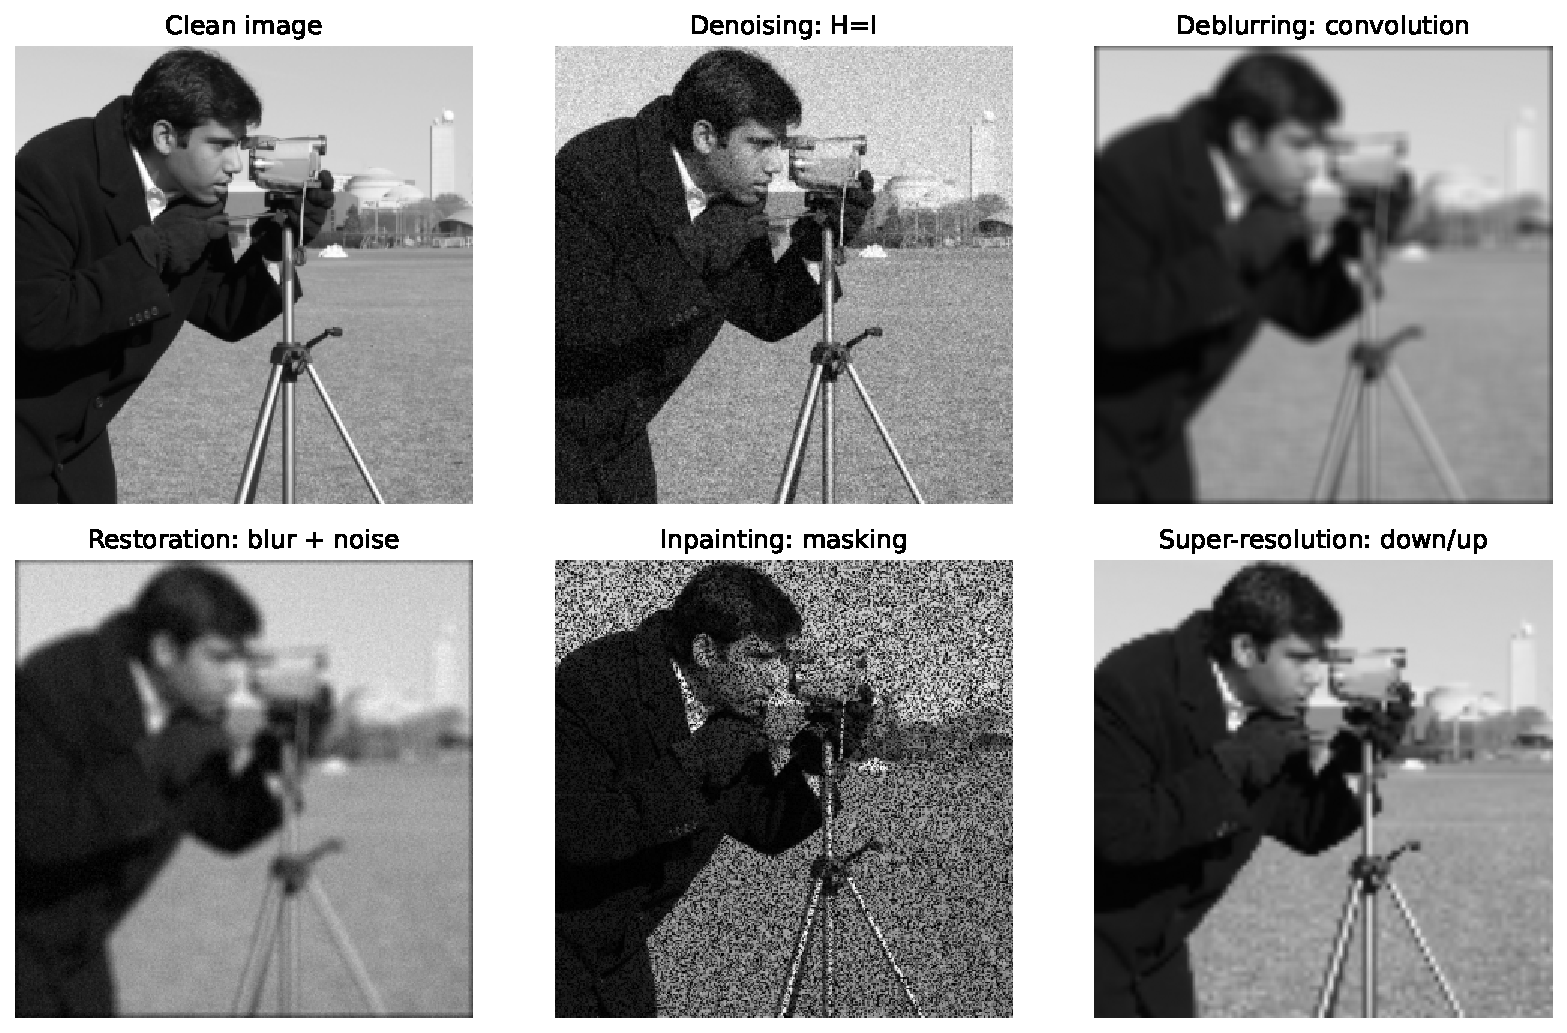
\includegraphics[width=.97\textwidth]{degradation_taxonomy.pdf}
\caption{چند مسئله ظاهراً متفاوت با تغییر عملگر پیشرو \(\op H\). حذف نویز فقط حالت \(\op H=\op I\) است.}
\label{fig:degradation-taxonomy}
\end{figure}

\begin{keybox}[سه محور قضاوت]
هر خروجی باید دست‌کم روی سه محور سنجیده شود:
\begin{enumerate}
\item \textbf{وفاداری به اندازه‌گیری:} آیا \(\op H(\widehat{\vect x})\) با \(\vect y\) سازگار است؟
\item \textbf{معقول‌بودن پیشینی:} آیا خروجی در کلاس تصاویر موردنظر قرار می‌گیرد؟
\item \textbf{فایده برای تصمیم:} آیا خروجی برای مشاهده، اندازه‌گیری یا وظیفه پایین‌دست مناسب است؟
\end{enumerate}
هیچ معیار منفردی هر سه را کامل اندازه نمی‌گیرد.
\end{keybox}

% =============================================================================
\section{صورت‌بندی یکپارچه: مدل پیشرو، درست‌نمایی و پیشین}
% =============================================================================

در حالت خطی گسسته می‌نویسیم
\begin{equation}
\vect y=\vect H\vect x+\vect n,
\qquad
\vect H\in\R^{m\times n},\quad
\vect x\in\R^n,\quad
\vect y\in\R^m.
\label{eq:linear-forward}
\end{equation}
عملگر \(\vect H\) می‌تواند همانی، کانولوشن تاری، ماسک نمونه‌برداری، کاهش ابعاد، تبدیل رادون یا ترکیبی از این‌ها باشد.
در مدل غیرخطی، \(\vect H\vect x\) با \(\op H(\vect x)\) جایگزین می‌شود.

اگر نویز گاوسی سفید باشد،
\begin{equation}
p(\vect y\mid\vect x)
=(2\pi\sigma^2)^{-m/2}
\exp\!\left(-\frac{1}{2\sigma^2}\norm{\vect y-\vect H\vect x}_2^2\right).
\end{equation}
پس منفی لگاریتم درست‌نمایی، تا یک ثابت، برابر است با
\begin{equation}
\mathcal D_{\mathrm G}(\vect x;\vect y)
=\frac{1}{2\sigma^2}\norm{\vect y-\vect H\vect x}_2^2.
\label{eq:gaussian-data-term}
\end{equation}
برای شمارش پواسون \(y_i\sim\Poisson((\vect H\vect x)_i)\)، جمله داده به صورت واگرایی تعمیم‌یافته کالبک--لایبلر درمی‌آید:
\begin{equation}
\mathcal D_{\mathrm P}(\vect x;\vect y)
=\sum_i\left[(\vect H\vect x)_i-y_i\log((\vect H\vect x)_i)\right],
\label{eq:poisson-data-term}
\end{equation}
با قرارداد مناسب برای \(y_i=0\). برای نویز لاپلاس، \(\ell_1\) و برای آلودگی‌های دنباله‌سنگین، هزینه‌های مقاوم مانند هیوبر یا دانشجویی مناسب‌ترند.

پیشین بیزی \(p(\vect x)\) را می‌توان به صورت انرژی نوشت:
\begin{equation}
p(\vect x)\propto \exp[-\lambda\mathcal R(\vect x)].
\end{equation}
در نتیجه برآورد \lr{MAP} برابر است با
\begin{equation}
\widehat{\vect x}_{\mathrm{MAP}}
=\argmin_{\vect x}\;\mathcal D(\vect x;\vect y)+\lambda\mathcal R(\vect x).
\label{eq:master-variational}
\end{equation}
این رابطه زبان مشترک بخش بزرگی از فصل است.

\begin{warningbox}
پارامتر \(\lambda\) «مقدار هموارسازی» صرف نیست؛ نسبت اعتماد به مدل داده و پیشین را تنظیم می‌کند.
اگر جمله داده با \(1/(2\sigma^2)\) مقیاس شده باشد، تفسیر \(\lambda\) با حالتی که این ضریب حذف شده متفاوت است.
گزارش \(\lambda\) بدون گزارش نرمال‌سازی و دامنه شدت قابل بازتولید نیست.
\end{warningbox}

\subsection{شرایط هادامار و علت نیاز به منظم‌سازی}

مسئله معکوس خوش‌وضع است اگر جواب وجود داشته باشد، یکتا باشد و به داده پیوسته وابسته باشد. در تجزیه مقدار منفرد
\begin{equation}
\vect H=\vect U\vect\Sigma\vect V\trans,
\end{equation}
معکوس کمترین مربعات، مؤلفه \(u_i\trans\vect y\) را بر \(\sigma_i\) تقسیم می‌کند. اگر \(\sigma_i\) کوچک باشد، نویز شدیداً تقویت می‌شود:
\begin{equation}
\widehat{\vect x}_{\mathrm{LS}}
=\sum_{i:\sigma_i>0}\frac{u_i\trans\vect y}{\sigma_i}v_i.
\label{eq:svd-inverse}
\end{equation}
منظم‌سازی عملاً ضرایب فیلتری \(\phi_i\) را وارد می‌کند:
\begin{equation}
\widehat{\vect x}_{\lambda}
=\sum_i \phi_i(\lambda,\sigma_i)\frac{u_i\trans\vect y}{\sigma_i}v_i.
\end{equation}
برای تیکانوف مرتبه صفر، \(\phi_i=\sigma_i^2/(\sigma_i^2+\lambda)\) است؛ بنابراین جهت‌های بدشرط سرکوب می‌شوند.

% =============================================================================
\section{برآوردگر مناسب از تابع خطر می‌آید}
% =============================================================================

در نظریه تصمیم، برای مشاهده \(\vect y\) و تصمیم \(a\)، خطر شرطی
\begin{equation}
\rho(a\mid\vect y)=\E[L(\vect X,a)\mid\vect Y=\vect y]
\end{equation}
است. برآورد بیز تصمیمی است که این خطر را کمینه کند.

\begin{theorem}[برآوردگر \lr{MMSE}]
اگر \(L(\vect x,a)=\norm{\vect x-a}_2^2\)، آنگاه
\begin{equation}
\widehat{\vect x}_{\mathrm{MMSE}}=\E[\vect X\mid\vect Y=\vect y].
\label{eq:mmse}
\end{equation}
\end{theorem}
\begin{proof}
با قرار دادن \(\vect m=\E[\vect X\mid\vect y]\) داریم
\begin{align}
\E[\norm{\vect X-a}^2\mid\vect y]
&=\E[\norm{\vect X-\vect m+\vect m-a}^2\mid\vect y]\\
&=\E[\norm{\vect X-\vect m}^2\mid\vect y]+\norm{\vect m-a}^2,
\end{align}
زیرا جمله متقاطع به دلیل تعریف میانگین شرطی صفر است. پس کمینه در \(a=\vect m\) رخ می‌دهد.
\end{proof}

برای هزینه قدرمطلق تک‌متغیره، میانه شرطی بهینه است. برای هزینه صفر--یک روی فضای گسسته، نما یا \lr{MAP} بهینه می‌شود.
از این رو \lr{MMSE} و \lr{MAP} عموماً یکسان نیستند. در پسین چندقله‌ای، میانگین ممکن است میان دو پاسخ معتبر قرار گیرد و تصویری مات تولید کند،
در حالی که \lr{MAP} فقط یک قله را انتخاب می‌کند.

\subsection{مثال گاوسی خطی}
اگر
\begin{equation}
\vect x\sim\Normal(\vect\mu_x,\vect C_x),\qquad
\vect n\sim\Normal(\mathbf{0},\vect C_n),
\end{equation}
آنگاه پسین گاوسی و میانگین شرطی برابر است با
\begin{equation}
\widehat{\vect x}
=\vect\mu_x+\vect C_x\vect H\trans
(\vect H\vect C_x\vect H\trans+\vect C_n)^{-1}
(\vect y-\vect H\vect\mu_x).
\label{eq:lmmse-general}
\end{equation}
این همان برآوردگر وینر تعمیم‌یافته است. در مدل کاملاً گاوسی، میانگین پسین و نما یکسان‌اند؛ این هم‌ارزی در پیشین‌های غیرگاوسی از بین می‌رود.

\begin{futurebox}
مدل مولد مدرن تقریب پیچیده‌ای از \(p(\vect x)\) یا گرادیان لگاریتم آن می‌آموزد، اما تصمیم نهایی همچنان باید مشخص کند
میانگین پسین، نمونه پسین، نما یا برآوردی با هزینه ادراکی مطلوب است. «شبکه قوی‌تر» این انتخاب نظری را حذف نمی‌کند.
\end{futurebox}

% =============================================================================
\section{فیلترهای خطی: از هموارسازی تا وینر}
% =============================================================================

\subsection{فیلتر خطی ناوردا نسبت به انتقال}

برای هسته \(h\)، خروجی
\begin{equation}
\widehat x[m,n]=(h*y)[m,n]
=\sum_{k,\ell}h[k,\ell]y[m-k,n-\ell]
\end{equation}
است. اگر \(\sum h=1\)، مؤلفه ثابت حفظ می‌شود. فیلتر میانگین و گاوسی نویز فرکانس بالا را کاهش می‌دهند،
ولی چون لبه نیز انرژی فرکانس بالا دارد، آن را هم تضعیف می‌کنند. این تضاد نخستین نمونه از مبادله سوگیری--واریانس است.

برای نویز سفید با واریانس \(\sigma_n^2\)، واریانس خروجی فیلتر خطی برابر است با
\begin{equation}
\Var[(h*n)[m,n]]=\sigma_n^2\sum_{k,\ell}h^2[k,\ell].
\label{eq:filtered-noise-var}
\end{equation}
پس پهن‌ترکردن هسته واریانس را کم می‌کند، اما سوگیری لبه‌ها را افزایش می‌دهد.

\subsection{استخراج فیلتر وینر از اصل تعامد}

در مدل فرکانسی
\begin{equation}
Y(\omega)=H(\omega)X(\omega)+N(\omega),
\end{equation}
برآورد خطی \(\widehat X=G Y\) را می‌خواهیم که
\(\E|X-GY|^2\) را کمینه کند. اصل تعامد می‌گوید خطا با داده نامرتبط است:
\begin{equation}
\E[(X-GY)Y^*]=0.
\end{equation}
بنابراین
\begin{equation}
G(\omega)=\frac{S_{XY}(\omega)}{S_{YY}(\omega)}.
\end{equation}
اگر سیگنال و نویز نامرتبط باشند،
\begin{equation}
G_{\mathrm W}(\omega)
=\frac{H^*(\omega)S_X(\omega)}{|H(\omega)|^2S_X(\omega)+S_N(\omega)}
=\frac{H^*(\omega)}{|H(\omega)|^2+S_N(\omega)/S_X(\omega)}.
\label{eq:wiener}
\end{equation}

\begin{figure}[H]
\centering
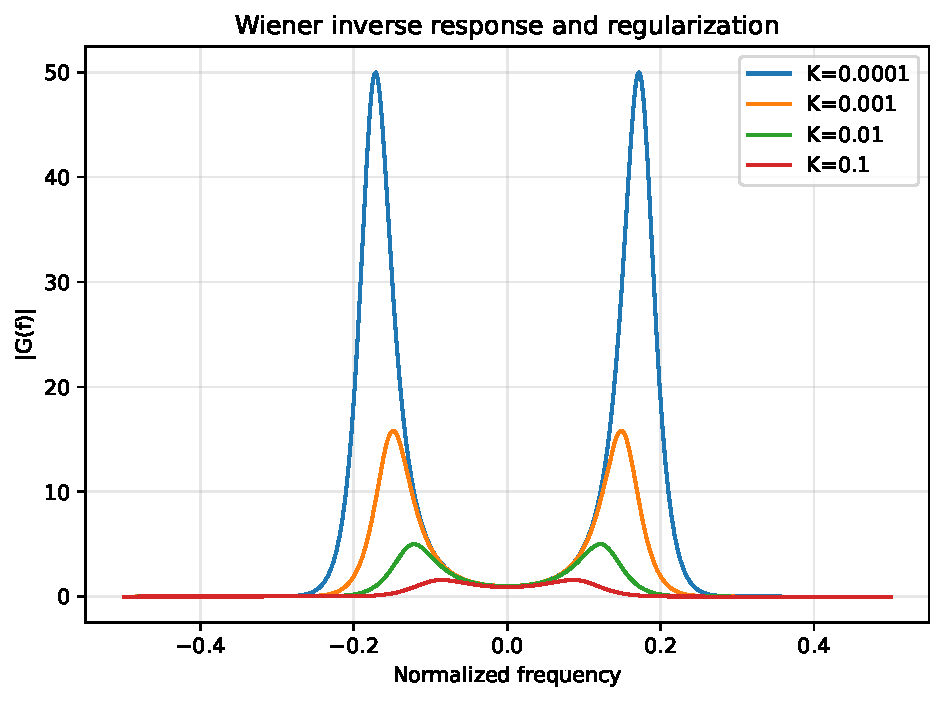
\includegraphics[width=.78\textwidth]{wiener_frequency_response.pdf}
\caption{پاسخ معکوس وینر. منظم‌سازی مانع انفجار بهره در فرکانس‌هایی می‌شود که \(H\) کوچک است.}
\label{fig:wiener-frequency}
\end{figure}

برای حذف نویز خالص \(H=1\)،
\begin{equation}
G_{\mathrm W}(\omega)=\frac{S_X(\omega)}{S_X(\omega)+S_N(\omega)},
\end{equation}
یعنی هر فرکانس به نسبت سیگنال به مجموع سیگنال و نویز وزن می‌گیرد. در ناحیه‌ای که \(S_X\gg S_N\)، بهره نزدیک یک و در ناحیه نویزغالب نزدیک صفر است.

\subsection{رابطه وینر و تیکانوف}

مسئله
\begin{equation}
\widehat{\vect x}
=\argmin_{\vect x}\frac{1}{2}\norm{\vect H\vect x-\vect y}_2^2
+\frac{\lambda}{2}\norm{\vect L\vect x}_2^2
\label{eq:tikhonov}
\end{equation}
معادله نرمال
\begin{equation}
(\vect H\trans\vect H+\lambda\vect L\trans\vect L)\widehat{\vect x}
=\vect H\trans\vect y
\end{equation}
را دارد. اگر عملگرها کانولوشنی باشند، در حوزه فوریه
\begin{equation}
\widehat X(\omega)
=\frac{H^*(\omega)}{|H(\omega)|^2+\lambda|L(\omega)|^2}Y(\omega).
\label{eq:tikhonov-frequency}
\end{equation}
این فرم از نظر جبری به وینر شبیه است. در دیدگاه بیزی، \(\norm{Lx}^2\) پیشین گاوسی با دقت متناسب با \(L^TL\) القا می‌کند.

\begin{warningbox}
فیلتر معکوس \(1/H\) در صفرها یا مقادیر کوچک \(H\) ناپایدار است. افزودن یک \(\epsilon\) دلخواه مشکل را پنهان می‌کند،
اما انتخاب علمی باید از سطح نویز، پیشین یا یک اصل منظم‌سازی مانند اختلاف، \lr{GCV} یا \lr{SURE} بیاید.
\end{warningbox}

% =============================================================================
\section{فیلترهای غیرخطی محلی و حفظ لبه}
% =============================================================================

\subsection{فیلتر میانه و آمار ترتیبی}

در پنجره \(\mathcal N_i\)، فیلتر میانه
\begin{equation}
\widehat x_i=\median\{y_j:j\in\mathcal N_i\}
\end{equation}
است. میانه کمینه‌کننده
\begin{equation}
\argmin_a\sum_{j\in\mathcal N_i}|y_j-a|
\end{equation}
است و از این رو در برابر چند مقدار پرت مقاوم‌تر از میانگین است. برای نویز نمک‌وفلفل، فیلتر میانه غالباً از هموارساز خطی بهتر است؛
اما در نویز گاوسی و بافت ریز الزاماً بهینه نیست.

\subsection{فیلتر دوطرفه}

فیلتر دوطرفه هم نزدیکی مکانی و هم شباهت شدت را وزن می‌دهد:
\begin{equation}
\widehat x_i=\frac{1}{Z_i}\sum_{j\in\mathcal N_i}
\exp\!\left(-\frac{\norm{p_i-p_j}^2}{2\sigma_s^2}
-\frac{(y_i-y_j)^2}{2\sigma_r^2}\right)y_j,
\label{eq:bilateral}
\end{equation}
که \(Z_i\) مجموع وزن‌ها است. پارامتر \(\sigma_s\) مقیاس مکانی و \(\sigma_r\) تحمل اختلاف شدت را کنترل می‌کند.
اگر \(\sigma_r\to\infty\)، فیلتر به گاوسی مکانی نزدیک می‌شود؛ اگر \(\sigma_r\) کوچک باشد، عبور از لبه محدود می‌شود.

\subsection{فیلتر هدایت‌شده}

در فیلتر هدایت‌شده فرض می‌شود خروجی در پنجره \(\omega_k\) رابطه محلی خطی با تصویر راهنما \(I\) دارد:
\begin{equation}
q_i=a_k I_i+b_k,\qquad i\in\omega_k.
\end{equation}
ضرایب از کمینه‌سازی
\begin{equation}
\sum_{i\in\omega_k}(a_kI_i+b_k-p_i)^2+\epsilon a_k^2
\end{equation}
به‌دست می‌آیند. حل بسته آن نشان می‌دهد که \(a_k\) با کوواریانس راهنما و ورودی و \(b_k\) با میانگین‌های محلی تعیین می‌شود.
این فیلتر برای انتقال لبه از راهنما مفید است، اما اگر راهنما ساختار نامربوط داشته باشد، اثر انتقال بافت رخ می‌دهد.

\begin{keybox}[اصل کلی فیلتر تطبیقی]
هموارسازی باید در امتداد ناحیه همگن قوی و در عبور از مرز ضعیف باشد. فیلتر دوطرفه این تصمیم را با اختلاف شدت،
فیلتر هدایت‌شده با مدل رگرسیون محلی، و روش‌های تغییراتی با وزن یا هندسه گرادیان اجرا می‌کنند.
\end{keybox}

% =============================================================================
\section{حذف نویز در حوزه تبدیل: موجک، تنکی و آستانه‌گذاری}
% =============================================================================

فرض کنید \(\vect W\) تبدیل متعامد و
\begin{equation}
\vect c=\vect W\vect x,
\qquad
\vect d=\vect W\vect y=\vect c+\vect\eta.
\end{equation}
برای نویز سفید گاوسی و \(W\) متعامد، \(\eta\) نیز سفید گاوسی با همان واریانس است. اگر تصویر در این پایه تنک باشد،
بسیاری از ضرایب حقیقی کوچک یا صفرند و می‌توان ضرایب نویزغالب را کاهش داد.

\subsection{آستانه سخت و نرم}
\begin{align}
\delta_{\mathrm{hard}}(d;\tau)&=d\,\mathbf 1(|d|>\tau),\\
\delta_{\mathrm{soft}}(d;\tau)&=\operatorname{sign}(d)\max(|d|-\tau,0).
\end{align}
آستانه نرم پیوسته است و دقیقاً عملگر پروگزیمال نرم \(\ell_1\) محسوب می‌شود:
\begin{equation}
\operatorname{prox}_{\lambda|\cdot|}(d)
=\argmin_c\frac12(c-d)^2+\lambda|c|
=\delta_{\mathrm{soft}}(d;\lambda).
\label{eq:soft-prox}
\end{equation}

\begin{figure}[H]
\centering
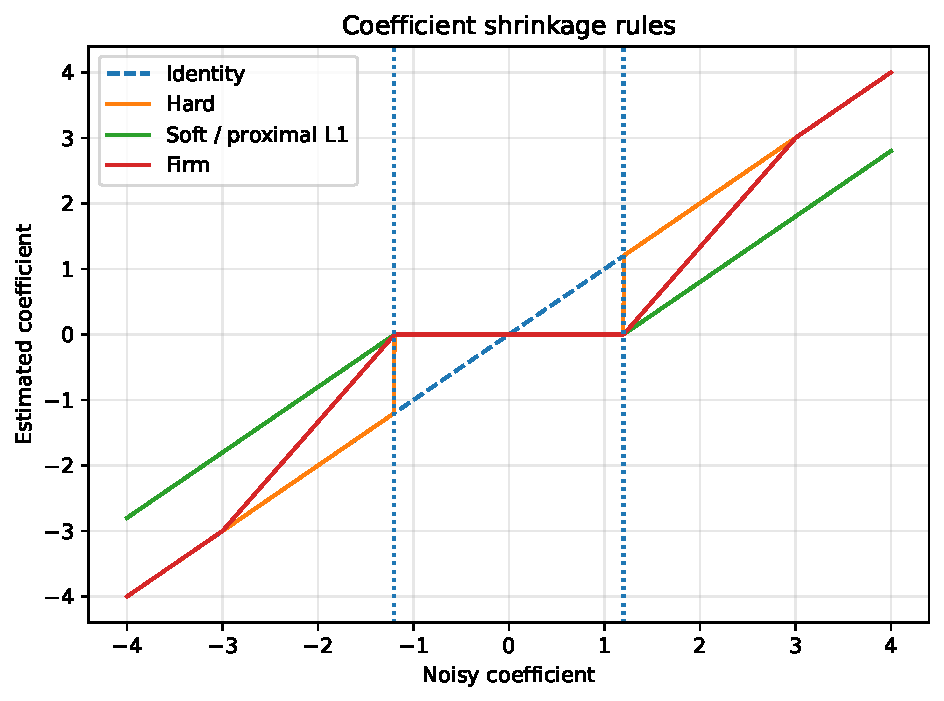
\includegraphics[width=.76\textwidth]{shrinkage_rules.pdf}
\caption{قواعد کاهش ضرایب. آستانه سخت ناپیوسته، آستانه نرم دارای سوگیری ثابت برای ضرایب بزرگ و آستانه \lr{firm} مصالحه‌ای میان آن‌ها است.}
\label{fig:shrinkage}
\end{figure}

\subsection{آستانه جهانی و \lr{SURE}}
اگر \(N\) ضریب نویز مستقل گاوسی داشته باشیم، آستانه جهانی دونوهیو--جانستون
\begin{equation}
\tau_{\mathrm{univ}}=\sigma\sqrt{2\log N}
\end{equation}
با احتمال بالا بیشینه نویز را پوشش می‌دهد، اما ممکن است بیش‌ازحد محافظه‌کار و هموارکننده باشد.
اصل برآورد بی‌طرفانه خطر استاین \lr{SURE} برای \(\vect y=\vect x+\sigma\vect z\) و تخمین‌گر تقریباً مشتق‌پذیر \(f\) می‌گوید
\begin{equation}
\mathrm{SURE}(f;\vect y)
=\norm{f(\vect y)-\vect y}^2+2\sigma^2\operatorname{div}f(\vect y)-n\sigma^2
\label{eq:sure}
\end{equation}
برآوردی بی‌طرف از خطر مربعی است. بنابراین پارامتر را می‌توان بدون تصویر پاک تنظیم کرد، مشروط بر درستی مدل گاوسی و محاسبه واگرایی.

\subsection{از تنکی ضرایب تا مدل فرهنگ لغت}
در مدل فرهنگ لغت
\begin{equation}
\vect y_i\approx\vect D\vect\alpha_i,
\qquad \norm{\vect\alpha_i}_0\ll p,
\end{equation}
هر وصله با تعداد کمی اتم بازسازی می‌شود. حل محدب رایج
\begin{equation}
\widehat{\vect\alpha}_i
=\argmin_{\vect\alpha}\frac12\norm{\vect y_i-\vect D\vect\alpha}_2^2+\lambda\norm{\vect\alpha}_1
\end{equation}
است. اگر \(D\) آموخته شود، داده خود پایه سازگار را تعیین می‌کند؛ اما هزینه یادگیری، خطر بیش‌برازش و وابستگی دامنه مطرح می‌شود.

% =============================================================================
\section{خودشباهتی غیرمحلی: از \lr{NLM} تا گروه‌بندی وصله‌ها}
% =============================================================================

تصویر طبیعی در نقاط دوردست نیز وصله‌های مشابه دارد. روش میانگین غیرمحلی برای پیکسل \(i\) می‌نویسد
\begin{equation}
\widehat x_i=\sum_{j\in\mathcal S_i}w_{ij}y_j,
\qquad
w_{ij}=\frac{1}{Z_i}\exp\!\left(-\frac{\norm{P_i\vect y-P_j\vect y}_{2,G}^2}{h^2}\right),
\label{eq:nlm}
\end{equation}
که \(P_i\) عملگر استخراج وصله و \(\norm{\cdot}_{2,G}\) فاصله وزن‌دار گاوسی است.
بر خلاف فیلتر دوطرفه که یک یا چند شدت را مقایسه می‌کند، \lr{NLM} هندسه کامل وصله را می‌سنجد.

\subsection{سوگیری فاصله وصله در حضور نویز}
اگر دو وصله پاک \(p_i,p_j\) و نویز مستقل گاوسی داشته باشند،
\begin{equation}
\E\norm{(p_i+n_i)-(p_j+n_j)}^2
=\norm{p_i-p_j}^2+2d\sigma^2,
\end{equation}
که \(d\) تعداد عناصر وصله است. پس فاصله خام دارای سوگیری وابسته به نویز است. در نویز شدید، انتخاب همسایه خطا می‌کند؛
این نکته انگیزه پیش‌فیلترکردن، تصحیح فاصله و تکرار چندمرحله‌ای است.

\subsection{گروه وصله و رتبه کم}
وصله‌های مشابه را ستون‌های ماتریس
\begin{equation}
\vect Y=[\vect y_{i_1},\ldots,\vect y_{i_K}]
=\vect X+\vect N
\end{equation}
قرار می‌دهیم. تکرار ساختار باعث می‌شود \(X\) تقریباً رتبه کم باشد. یک مدل پایه
\begin{equation}
\widehat{\vect X}
=\argmin_{\vect X}\frac12\norm{\vect Y-\vect X}_F^2+\lambda\norm{\vect X}_*
\end{equation}
است که حل آن آستانه‌گذاری نرم مقادیر منفرد است.

\begin{figure}[H]
\centering
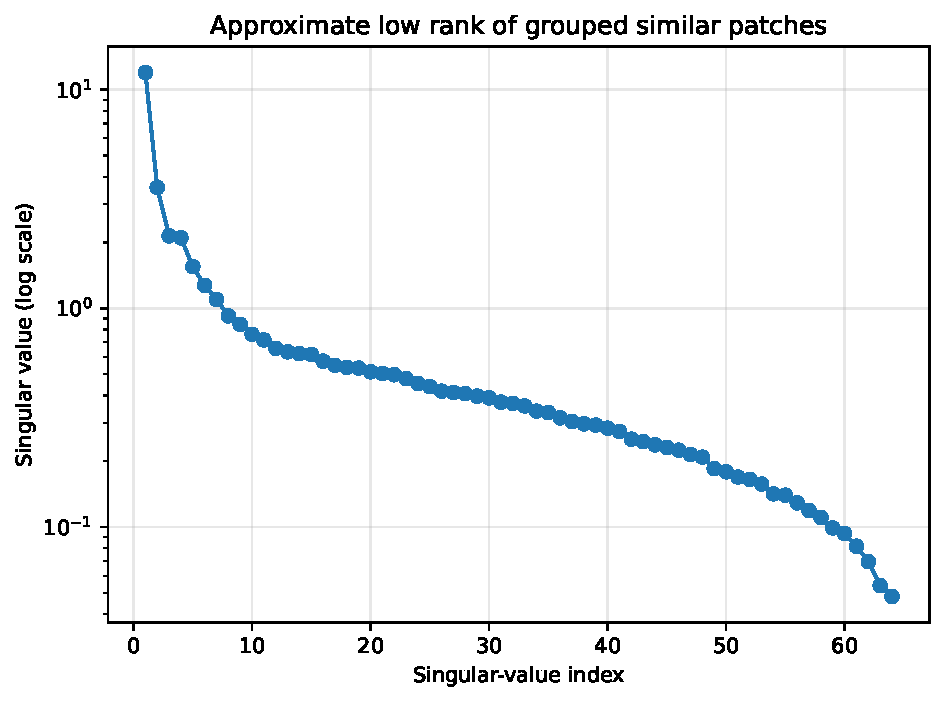
\includegraphics[width=.73\textwidth]{patch_group_singular_values.pdf}
\caption{افت مقادیر منفرد یک گروه وصله مشابه. ساختار تکراری در ماتریس گروهی به رتبه مؤثر پایین منجر می‌شود.}
\label{fig:patch-rank}
\end{figure}

\subsection{منطق \lr{BM3D}}
\lr{BM3D} سه ایده را ترکیب می‌کند: جست‌وجوی بلوک‌های مشابه، چیدن آن‌ها در آرایه سه‌بعدی، و کاهش ضرایب در یک تبدیل سه‌بعدی.
مرحله نخست با آستانه سخت یک برآورد پایه می‌دهد؛ مرحله دوم با گروه‌بندی بر اساس برآورد پایه و فیلتر وینر، خروجی را پالایش می‌کند.
نکته مهم این است که قدرت روش فقط از یک فیلتر نیست؛ از \textbf{همکاری} میان خودشباهتی، تبدیل تنک و تجمیع وزن‌دار می‌آید \cite{dabov2007bm3d}.

\begin{keybox}[یک تفسیر واحد]
موجک تنکی را در یک پایه ثابت می‌جوید؛ فرهنگ لغت پایه را از داده می‌آموزد؛ \lr{NLM} میانگین‌گیری روی منیفلد وصله انجام می‌دهد؛
و روش‌های رتبه‌کم وصله‌های مشابه را در یک زیرفضای کم‌بعد قرار می‌دهند. همه آن‌ها تلاش می‌کنند درجه آزادی مؤثر تصویر را از تعداد پیکسل‌ها کمتر کنند.
\end{keybox}

% =============================================================================
\section{بازسازی تغییراتی: هزینه داده و هندسه پیشین}
% =============================================================================

\subsection{پیشین همواری درجه دوم}
مدل
\begin{equation}
\min_x\frac12\norm{Hx-y}^2+\frac\lambda2\norm{\nabla x}^2
\end{equation}
محدب و قابل حل است، اما لبه را نیز جریمه می‌کند. در یک بعد، \(\norm{Dx}^2\) تغییرات زیاد را به‌طور درجه دوم پرهزینه می‌کند و بنابراین گذار تیز را پخش می‌سازد.

\subsection{تغییرات کلی}
برای تصویر پیوسته، تغییرات کلی همسانگرد
\begin{equation}
\operatorname{TV}(x)=\int_\Omega\norm{\nabla x(\vect r)}_2\,d\vect r
\end{equation}
و در شبکه گسسته
\begin{equation}
\operatorname{TV}(\vect x)=\sum_i\sqrt{(D_x\vect x)_i^2+(D_y\vect x)_i^2}
\label{eq:tv}
\end{equation}
است. مدل \lr{ROF} برای نویز گاوسی
\begin{equation}
\widehat x=\argmin_x\frac12\norm{x-y}_2^2+\lambda\operatorname{TV}(x)
\label{eq:rof}
\end{equation}
است \cite{rudin1992tv}.

در ناحیه‌ای که \(\nabla x\neq0\)، معادله اویلر--لاگرانژ رسمی
\begin{equation}
x-y-\lambda\operatorname{div}\!\left(\frac{\nabla x}{\norm{\nabla x}_2}\right)=0
\label{eq:tv-euler}
\end{equation}
است. عبارت واگرایی نرمال گرادیان با خمیدگی خطوط تراز ارتباط دارد و هموارسازی را درون ناحیه قوی‌تر از عبور از لبه می‌کند.

\begin{figure}[H]
\centering
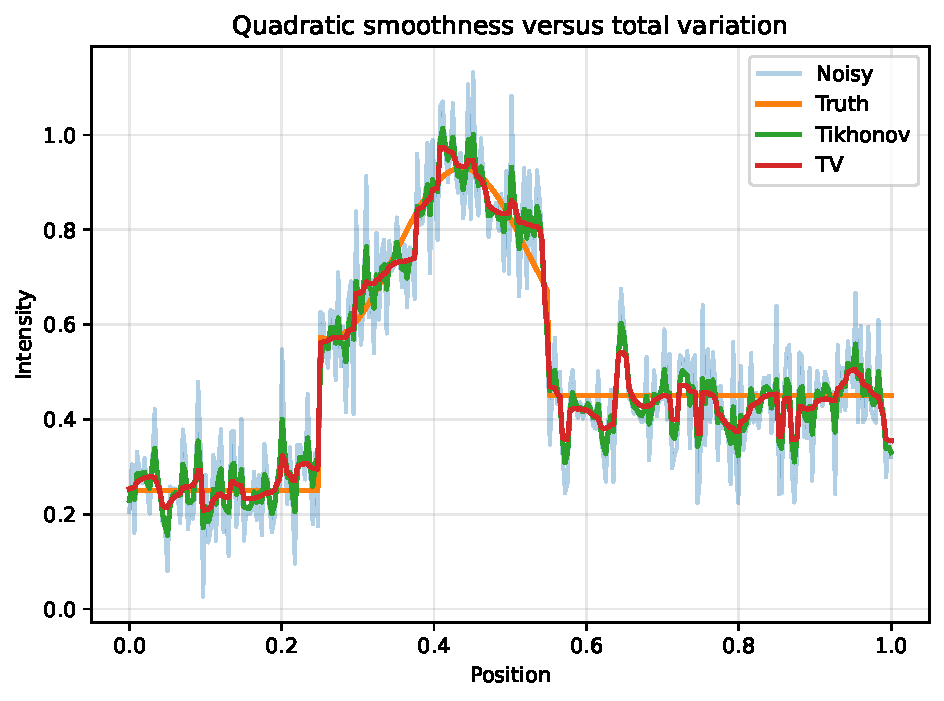
\includegraphics[width=.9\textwidth]{tikhonov_vs_tv_1d.pdf}
\caption{مقایسه همواری درجه دوم و \lr{TV}. تیکانوف گذار را پخش می‌کند؛ \lr{TV} لبه را حفظ می‌کند ولی ممکن است پدیده پلکانی ایجاد کند.}
\label{fig:tikhonov-tv}
\end{figure}

\subsection{ناهمواری، پلکانی‌شدن و مدل‌های مرتبه بالاتر}
\lr{TV} گرادیان تنک را ترجیح می‌دهد و تصویر را قطعه‌ای ثابت می‌بیند. در رمپ‌های نرم، این فرض به نواحی تخت و پرش‌های مصنوعی منجر می‌شود.
راه‌حل‌ها شامل هیوبرکردن نرم گرادیان، \lr{TGV}، منظم‌سازی هسین و ترکیب چندمقیاسی‌اند. برای مثال
\begin{equation}
\operatorname{TGV}^2_{\alpha_0,\alpha_1}(x)
=\min_{\vect w}\alpha_1\norm{\nabla x-\vect w}_1+\alpha_0\norm{\mathcal E\vect w}_1
\end{equation}
می‌تواند نواحی قطعه‌ای خطی را بهتر مدل کند.

\subsection{هزینه داده باید با نویز هماهنگ باشد}
\begin{center}
\begin{tabularx}{.96\textwidth}{>{\raggedleft\arraybackslash}p{2.4cm} >{\centering\arraybackslash}p{3.2cm} X}
\toprule
مدل مشاهده & جمله داده & نکته \\
\midrule
گاوسی & \(\frac12\norm{Hx-y}_2^2\) & مناسب خطای جمع‌شونده با واریانس ثابت \\
لاپلاس & \(\norm{Hx-y}_1\) & مقاوم‌تر به پرت‌های متقارن \\
پواسون & \(\sum_i[(Hx)_i-y_i\log(Hx)_i]\) & نیازمند مثبت‌بودن شدت پیش‌بینی‌شده \\
نمک‌وفلفل & \(\ell_1\)، مدل ماسک یا متغیر پرت & مدل گاوسی می‌تواند پرت را روی کل تصویر پخش کند \\
اسپکل & هزینه در حوزه لگاریتم یا درست‌نمایی گاما & تبدیل لگاریتم سوگیری و مشکل صفر ایجاد می‌کند \\
\bottomrule
\end{tabularx}
\end{center}

% =============================================================================
\section{روش‌های پروگزیمال: از فرمول تا الگوریتم قابل اجرا}
% =============================================================================

برای
\begin{equation}
\min_x F(x)=f(x)+g(x),
\end{equation}
که \(f\) هموار با گرادیان لیپ‌شیتز و \(g\) محدب ولی شاید ناهموار است، عملگر پروگزیمال
\begin{equation}
\operatorname{prox}_{\gamma g}(v)
=\argmin_x\left\{g(x)+\frac{1}{2\gamma}\norm{x-v}^2\right\}
\end{equation}
تعریف می‌شود.

\subsection{گرادیان پروگزیمال و \lr{ISTA}}
\begin{equation}
x^{k+1}=\operatorname{prox}_{\gamma g}
\left(x^k-\gamma\nabla f(x^k)\right),
\qquad 0<\gamma<2/L.
\label{eq:ista}
\end{equation}
برای \(g(x)=\lambda\norm{x}_1\)، پروگزیمال همان آستانه نرم است. \lr{FISTA} با یک جمله مومنتوم نرخ تابع هدف را از مرتبه \(O(1/k)\) به \(O(1/k^2)\) در حالت محدب بهبود می‌دهد.

\begin{figure}[H]
\centering
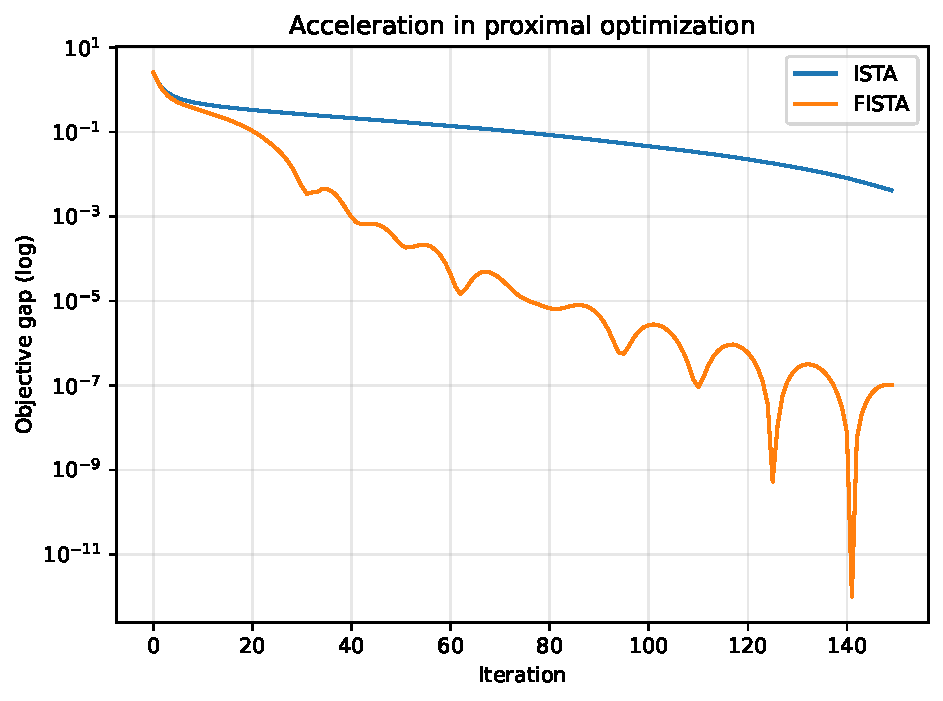
\includegraphics[width=.76\textwidth]{ista_fista_convergence.pdf}
\caption{نمونه همگرایی \lr{ISTA} و \lr{FISTA} در یک مسئله درجه‌دو به‌علاوه \(\ell_1\). شتاب در عمل می‌تواند نوسان نیز ایجاد کند.}
\label{fig:ista-fista}
\end{figure}

\subsection{تفکیک متغیر و \lr{ADMM}}
برای
\begin{equation}
\min_x f(x)+g(Kx)
\end{equation}
متغیر \(z=Kx\) وارد می‌کنیم. نسخه مقیاس‌شده \lr{ADMM}:
\begin{align}
x^{k+1}&=\argmin_x f(x)+\frac\rho2\norm{Kx-z^k+u^k}^2,\\
z^{k+1}&=\operatorname{prox}_{g/\rho}(Kx^{k+1}+u^k),\\
u^{k+1}&=u^k+Kx^{k+1}-z^{k+1}.
\end{align}
در \lr{TV}، یکی از زیرمسئله‌ها خطی و دیگری کاهش برداری گرادیان است. باقیمانده اولیه
\(r^k=Kx^k-z^k\) و باقیمانده دوگان برای توقف و تنظیم \(\rho\) اهمیت دارند.

\subsection{الگوریتم اولیه--دوگان}
نمایش دوگان
\begin{equation}
\operatorname{TV}(x)=\max_{\norm{p_i}\le1}\inner{\nabla x}{p}
\end{equation}
به الگوریتم‌های اولیه--دوگان منجر می‌شود که از حل دستگاه بزرگ اجتناب می‌کنند. شرط پایه گام‌ها معمولاً
\begin{equation}
\tau\sigma\norm{K}^2<1
\end{equation}
است. این روش‌ها برای مدل‌های ترکیبی و قیود مثبت‌بودن بسیار مناسب‌اند.

\begin{codecontract}
در کد، باید دقیقاً مشخص شود که \(f\)، \(g\)، \(K\)، پروگزیمال، گام‌ها و معیار توقف کدام‌اند.
نام‌گذاری تابعی مانند \lr{restore()} بدون ثبت این قرارداد، امکان بررسی صحت علمی را از بین می‌برد.
\end{codecontract}

% =============================================================================
\section{سه مسئله بنیادین بازسازی: تاری، فقدان و تفکیک‌پذیری}
% =============================================================================

\subsection{رفع تاری}
برای تاری ناوردا
\begin{equation}
y=h*x+n.
\end{equation}
شرایط مرزی اهمیت اساسی دارند. کانولوشن دوری، بازتابی و صفرگذاری سه ماتریس \(H\) متفاوت می‌سازند.
استفاده از \lr{FFT} اغلب کانولوشن دوری را ضمنی فرض می‌کند؛ اگر تصویر واقعی چنین مرزی نداشته باشد، حلقه‌های مرزی ایجاد می‌شود.

\begin{figure}[H]
\centering
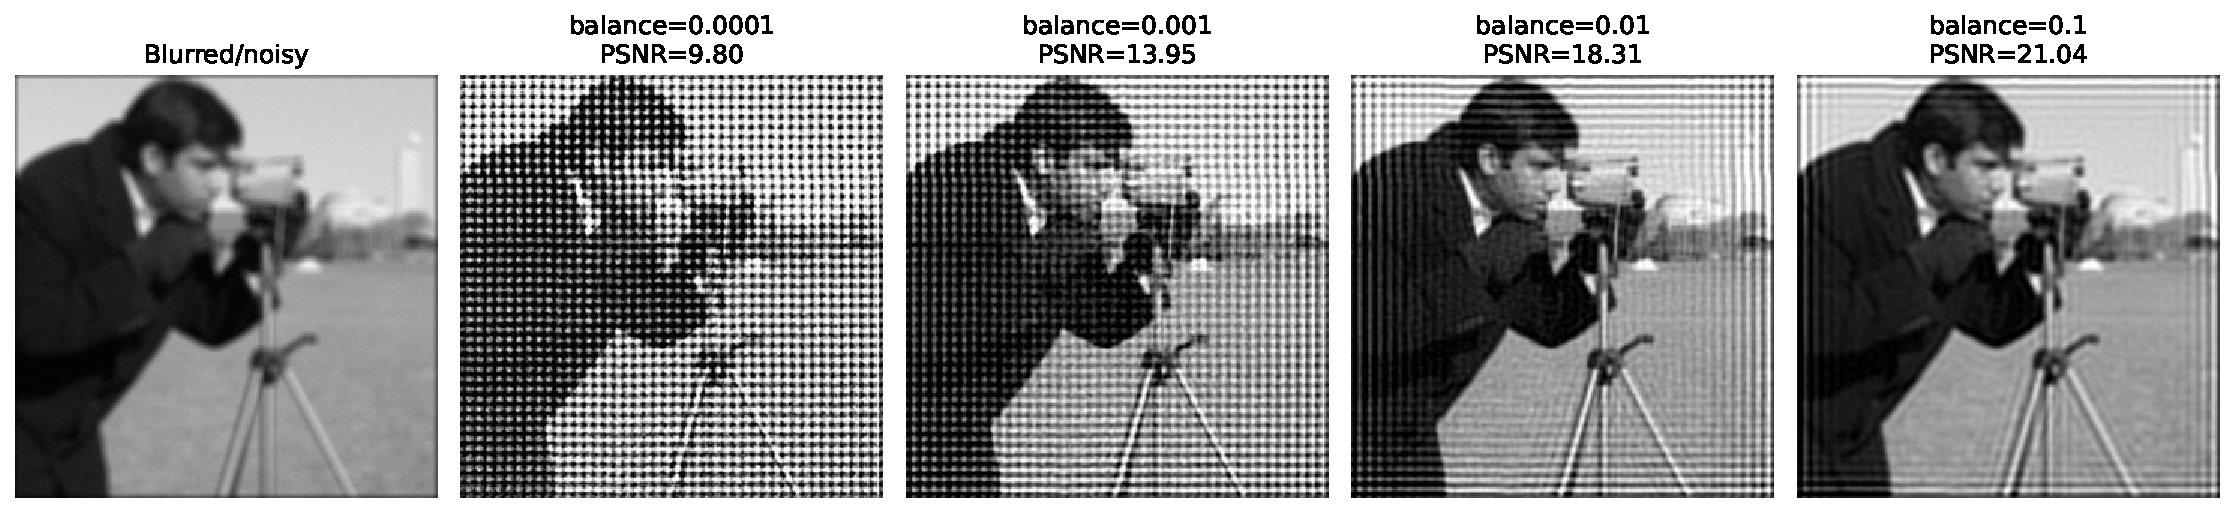
\includegraphics[width=.98\textwidth]{deblurring_regularization_path.pdf}
\caption{مسیر منظم‌سازی در رفع تاری. منظم‌سازی بسیار کم نویز و حلقه را تقویت می‌کند و منظم‌سازی زیاد جزئیات را حذف می‌کند.}
\label{fig:deblur-path}
\end{figure}

\subsection{درون‌پرکردن}
اگر \(M\) ماسک قطری مشاهده باشد،
\begin{equation}
y=Mx+n.
\end{equation}
در پیکسل‌های مفقود، جمله داده هیچ اطلاعات مستقیمی نمی‌دهد و تمام پاسخ از پیشین و ساختار پیرامون می‌آید.
این مسئله مثال روشنی است که چرا خروجی محتمل الزاماً حقیقت تاریخی نیست.

\subsection{ابرتفکیک}
مدل ساده
\begin{equation}
y=SHx+n
\end{equation}
است؛ \(H\) تاری اپتیکی و \(S\) زیرنمونه‌برداری است. فرکانس‌های حذف‌شده قابل بازیابی یکتا نیستند.
روش اعوجاج‌محور معمولاً میانگین بافت‌های ممکن را می‌دهد؛ روش مولد یک بافت محتمل تولید می‌کند. این دو هدف باید در گزارش جدا شوند.

\subsection{رفع تاری کور و شناساپذیری}
در تاری کور، هم \(x\) و هم هسته \(h\) مجهول‌اند:
\begin{equation}
y=h*x+n.
\end{equation}
ابهام مقیاس \((ch)*(x/c)=h*x\)، ابهام انتقال و جواب ضربه‌ای از مشکلات پایه‌اند. قیود
\begin{equation}
h\ge0,\qquad \sum_i h_i=1
\end{equation}
و پیشین‌های متفاوت برای تصویر و هسته لازم‌اند. حل متناوب
\begin{align}
x^{k+1}&=\argmin_x \mathcal D(h^k*x,y)+\lambda R(x),\\
h^{k+1}&=\argmin_h \mathcal D(h*x^{k+1},y)+\gamma Q(h)
\end{align}
غیرمحدب است و به مقداردهی اولیه حساس می‌ماند.

% =============================================================================
\section{انتخاب پارامتر: اختلاف، اعتبارسنجی، \lr{GCV} و \lr{SURE}}
% =============================================================================

انتخاب پارامتر بخشی از الگوریتم است، نه جزئیات جانبی. چهار سناریو:
\begin{enumerate}
\item \textbf{تصویر پاک موجود:} اعتبارسنجی روی مجموعه‌ای جدا از آزمون؛
\item \textbf{سطح نویز معلوم:} اصل اختلاف موروزوف، یعنی \(\norm{H\hat x-y}^2\approx m\sigma^2\)؛
\item \textbf{برآوردگر خطی:} اعتبارسنجی متقاطع تعمیم‌یافته؛
\item \textbf{نویز گاوسی و تخمین‌گر مشتق‌پذیر:} \lr{SURE} یا تقریب مونت‌کارلو واگرایی.
\end{enumerate}

برای تخمین‌گر خطی \(\widehat y=A_\lambda y\)،
\begin{equation}
\operatorname{GCV}(\lambda)
=\frac{\norm{(I-A_\lambda)y}^2/m}
{\left[1-\trace(A_\lambda)/m\right]^2}.
\end{equation}
مخرج درجه آزادی مؤثر مدل را جبران می‌کند.

\begin{figure}[H]
\centering
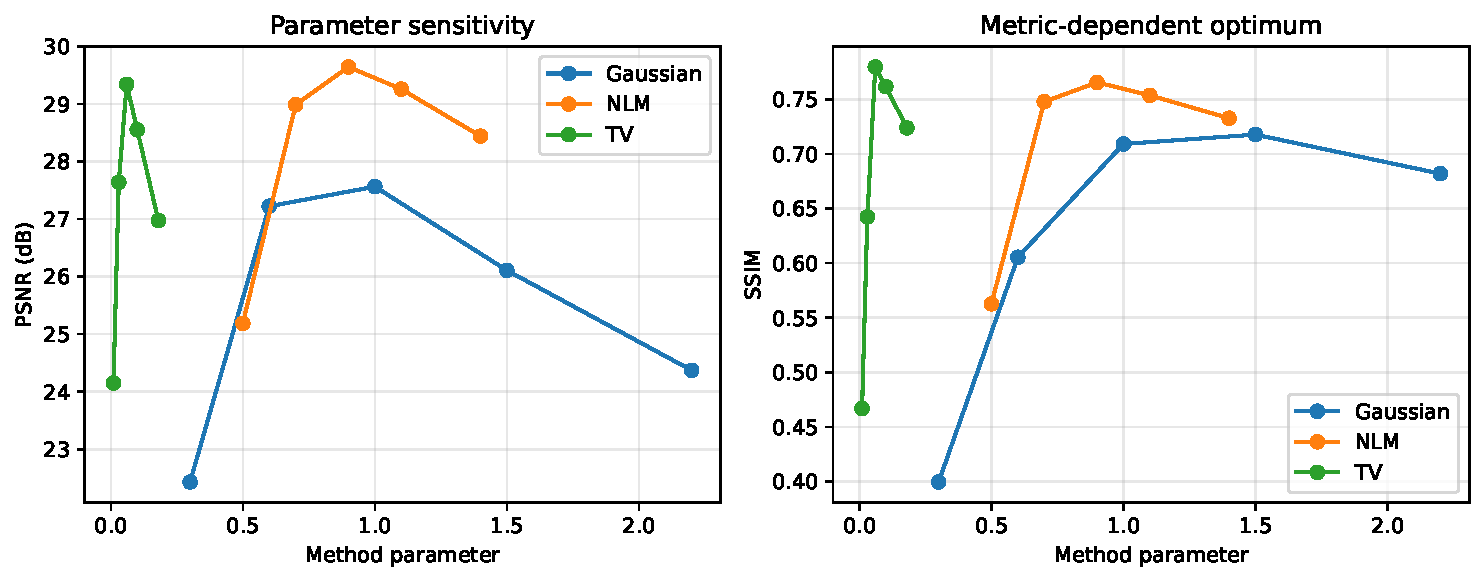
\includegraphics[width=.96\textwidth]{parameter_sensitivity.pdf}
\caption{حساسیت روش‌ها به پارامتر. حتی برای یک داده ثابت، پارامتر بهینه \lr{PSNR} و \lr{SSIM} می‌تواند متفاوت باشد.}
\label{fig:param-sensitivity}
\end{figure}

\begin{warningbox}
انتخاب پارامتر روی همان تصویر یا همان مجموعه‌ای که نتیجه نهایی روی آن گزارش می‌شود، برآورد عملکرد را خوش‌بینانه می‌کند.
در مقایسه روش‌ها باید بودجه جست‌وجوی ابرپارامتر و اطلاعات در دسترس برای همه روش‌ها منصفانه باشد.
\end{warningbox}

% =============================================================================
\section{یادگیری نظارت‌شده: شبکه به‌عنوان برآوردگر داده‌محور}
% =============================================================================

مجموعه زوج‌های \((y_i,x_i)\) و شبکه \(f_\theta\) را در نظر بگیرید:
\begin{equation}
\widehat\theta=\argmin_\theta\frac1N\sum_{i=1}^N L(f_\theta(y_i),x_i).
\end{equation}
با هزینه مربعی و داده کافی، تابع بهینه به میانگین شرطی \(\E[X\mid Y=y]\) نزدیک می‌شود؛ با \(\ell_1\)، به میانه شرطی مؤلفه‌ای نزدیک می‌شود.
بنابراین انتخاب هزینه همچنان تصمیم آماری است.

\subsection{یادگیری باقیمانده}
در حذف نویز جمع‌شونده، شبکه می‌تواند نویز را تخمین بزند:
\begin{equation}
\widehat n_\theta(y)\approx y-x,
\qquad
\widehat x=y-\widehat n_\theta(y).
\end{equation}
این ایده در \lr{DnCNN} با کانولوشن عمیق، نرمال‌سازی دسته‌ای و یادگیری باقیمانده به یک خط مبنای مهم تبدیل شد \cite{zhang2017dncnn}.
از نظر بهینه‌سازی، هدف باقیمانده اغلب نزدیک‌تر به صفر و از نظر آماری ساده‌تر از نگاشت کامل تصویر است.

\subsection{نقشه نویز و مدل کور}
اگر سطح نویز \(\sigma\) معلوم باشد، می‌توان آن را به شبکه داد:
\begin{equation}
\widehat x=f_\theta(y,\sigma).
\end{equation}
در مدل مکانی، نقشه \(M_\sigma(i)\) وارد می‌شود. در مدل کور، شبکه باید هم تخریب را استنباط و هم تصویر را بازسازی کند؛
این انعطاف می‌تواند به ابهام و شکست خارج از توزیع منجر شود.

\subsection{توابع هزینه}
\begin{align}
L_{\mathrm{pix}}&=\norm{\widehat x-x}_1\quad\text{یا}\quad\norm{\widehat x-x}_2^2,\\
L_{\mathrm{grad}}&=\norm{\nabla\widehat x-\nabla x}_1,\\
L_{\mathrm{perc}}&=\sum_\ell\norm{\phi_\ell(\widehat x)-\phi_\ell(x)}^2,\\
L_{\mathrm{adv}}&=\text{هزینه خصمانه برای نزدیک‌کردن توزیع خروجی به تصویر طبیعی}.
\end{align}
هزینه ادراکی می‌تواند بافت خوشایندتر بسازد، اما تضمین اندازه‌گیری پیکسلی را کاهش دهد. برای کاربرد علمی باید جمله سازگاری داده مستقل حفظ شود.

\subsection{از کانولوشن تا ترنسفورمر}
شبکه‌های کانولوشنی سوگیری محلی و ناوردایی انتقال دارند. ترنسفورمرها وابستگی دوربرد را با توجه مدل می‌کنند،
ولی توجه سراسری روی تصویر بزرگ هزینه درجه دوم دارد. \lr{SwinIR} از پنجره‌های انتقال‌یافته و \lr{Restormer} از طراحی توجه کارآمد برای بازسازی وضوح بالا استفاده می‌کنند \cite{liang2021swinir,zamir2022restormer}.
نکته آموزشی مهم این است که عملکرد قوی لزوماً از پیچیدگی فعال‌ساز نمی‌آید؛ \lr{NAFNet} نشان داد یک خط مبنای ساده و مهندسی‌شده نیز می‌تواند رقابتی باشد \cite{chen2022nafnet}.

\begin{futurebox}
روند پژوهش از «یک شبکه برای یک تخریب معلوم» به مدل‌های کور، همه‌کاره و پایه بازسازی حرکت کرده است.
مدل‌هایی مانند \lr{PromptIR} از نمایش تخریب برای هدایت بازسازی استفاده می‌کنند و کارهای جدیدتر مقیاس داده و ظرفیت را افزایش داده‌اند.
اما مسئله دهه آینده فقط افزایش اندازه نیست: کالیبراسیون عدم‌قطعیت، کنترل توهم، هزینه انرژی، سازگاری حسگر و ارزیابی خارج از توزیع تعیین‌کننده‌اند \cite{potlapalli2023promptir,li2025foundir}.
\end{futurebox}

% =============================================================================
\section{شبکه‌های بازشده: الگوریتم تکراری به معماری قابل یادگیری}
% =============================================================================

اگر یک گام گرادیان پروگزیمال را بنویسیم
\begin{equation}
x^{k+1}=\mathcal P_{\theta_k}\left(x^k-\gamma_k H\trans(Hx^k-y)\right),
\end{equation}
می‌توان تعداد ثابتی گام را به لایه‌های شبکه تبدیل کرد و \(\gamma_k\)، آستانه‌ها، تبدیل‌ها یا حتی پروگزیمال را آموخت.
این رویکرد \lr{algorithm unrolling} سه مزیت دارد:
\begin{enumerate}
\item سازگاری داده به‌طور صریح در معماری حضور دارد؛
\item تعداد مراحل و هزینه محاسباتی قابل کنترل است؛
\item پارامترها تفسیرپذیرتر از شبکه جعبه‌سیاه‌اند.
\end{enumerate}
با این حال، تضمین الگوریتم اصلی پس از آزادکردن پارامترها الزاماً حفظ نمی‌شود. شبکه ممکن است فقط برای توزیع آموزشی و تعداد مراحل مشخص خوب باشد.

\subsection{تفکیک نقش‌ها}
یک بلوک بازشده بهتر است سه جزء را جدا کند:
\begin{equation}
\text{حالت جدید}
=\text{سازگاری داده} + \text{پیشین آموخته‌شده} + \text{حافظه/شتاب}.
\end{equation}
این تفکیک در آزمایش حذف مؤلفه و انتقال میان عملگرها اهمیت دارد.

% =============================================================================
\section{\lr{Plug-and-Play} و \lr{RED}: حذف نویز به‌عنوان پیشین}
% =============================================================================

در \lr{ADMM} برای مسئله \(f(x)+\lambda R(x)\)، گام \(z\) یک پروگزیمال از \(R\) است. ایده \lr{Plug-and-Play}
آن است که این پروگزیمال با یک حذف‌کننده نویز \(D_\sigma\) جایگزین شود:
\begin{align}
x^{k+1}&=\argmin_x f(x)+\frac\rho2\norm{x-z^k+u^k}^2,\\
z^{k+1}&=D_\sigma(x^{k+1}+u^k),\\
u^{k+1}&=u^k+x^{k+1}-z^{k+1}.
\label{eq:pnp-admm}
\end{align}
این چارچوب اجازه می‌دهد یک حذف‌کننده قوی برای مسائل مختلف \(H\) استفاده شود، بدون آموزش جداگانه برای هر عملگر.

\subsection{آیا هر حذف‌کننده یک پروگزیمال است؟}
خیر. برای اینکه \(D\) پروگزیمال یک تابع محدب باشد، خواص ساختاری مانند firmly nonexpansive بودن لازم است.
یک شبکه عمومی ممکن است چنین خاصیتی نداشته باشد. بنابراین تفسیر \lr{PnP} بهتر است به‌صورت نقطه ثابت یا تعادل اجماع نوشته شود:
\begin{equation}
x^*=F(x^*),
\end{equation}
نه الزاماً کمینه‌ساز یک انرژی صریح.

در \lr{RED} منظم‌ساز پیشنهادی
\begin{equation}
R_{\mathrm{RED}}(x)=\frac12x\trans(x-D(x))
\end{equation}
است. تحت شرایطی مانند همگنی محلی و تقارن ژاکوبین، گرادیان آن \(x-D(x)\) می‌شود؛ این شرایط برای شبکه‌های دلخواه خودکار نیستند.
تحلیل‌های جدیدتر نشان می‌دهند که رفتار \lr{PnP/RED} را می‌توان از طریق مجموعه نقاط ثابت حذف‌کننده و کران‌های بازیابی مطالعه کرد \cite{venkatakrishnan2013pnp,romano2017red,liu2021recovery}.

\begin{keybox}[چرا این بخش برای دهه آینده مهم است؟]
\lr{PnP} مرز «مدل‌محور» و «داده‌محور» را می‌شکند: عملگر فیزیکی در جمله داده باقی می‌ماند و پیشین با حذف‌کننده آموخته می‌شود.
این الگو در تصویربرداری پزشکی، میکروسکوپی، نجومی و سنجش از دور قابل انتقال‌تر از شبکه انتهابه‌انتها برای یک دستگاه ثابت است.
\end{keybox}

% =============================================================================
\section{پیشین امتیاز و مدل انتشار: از حذف نویز تا نمونه‌گیری پسین}
% =============================================================================

\subsection{تابع امتیاز و هویت توییدی}
اگر \(x\sim p_X\) و \(y=x+\sigma z\)، آنگاه برای چگالی هموارشده \(p_\sigma(y)\)، هویت توییدی می‌گوید
\begin{equation}
\E[X\mid Y=y]=y+\sigma^2\nabla_y\log p_\sigma(y).
\label{eq:tweedie}
\end{equation}
پس حذف‌کننده \lr{MMSE} اطلاعاتی از امتیاز \(s_\sigma(y)=\nabla_y\log p_\sigma(y)\) می‌دهد:
\begin{equation}
s_\sigma(y)=\frac{D_\sigma(y)-y}{\sigma^2}.
\end{equation}
مدل‌های مبتنی بر امتیاز این میدان برداری را در سطوح نویز مختلف می‌آموزند و با یک فرایند معکوس از نویز به تصویر حرکت می‌کنند.

\subsection{پسین در مسئله معکوس}
\begin{equation}
\nabla_x\log p(x\mid y)
=\nabla_x\log p(x)+\nabla_x\log p(y\mid x).
\label{eq:posterior-score}
\end{equation}
این تجزیه جذاب است: مدل انتشار امتیاز پیشین را می‌دهد و مدل فیزیکی گرادیان درست‌نمایی را.
در نویز گاوسی خطی
\begin{equation}
\nabla_x\log p(y\mid x)=\frac{1}{\sigma_n^2}H\trans(y-Hx).
\end{equation}
در عمل، اعمال این راهنمایی در زمان‌های نویزی نیازمند تقریب \(p(y\mid x_t)\) است. روش‌هایی مانند \lr{DPS} با تقریب تصویر پاک از حالت میانی،
برای مسائل خطی و غیرخطی نویزی نمونه‌گیری تقریبی انجام می‌دهند \cite{chung2023dps}.

\subsection{برآورد نقطه‌ای در برابر نمونه پسین}
در مسئله شدیداً کم‌اطلاع، یک پاسخ یکتا وانمودکردن قطعیت است. نمونه‌های
\begin{equation}
x^{(1)},\ldots,x^{(K)}\sim p(x\mid y)
\end{equation}
می‌توانند تنوع پاسخ‌های سازگار را نشان دهند. میانگین نمونه‌ها، واریانس پیکسلی و بازه ویژگی‌های اندازه‌گیری‌شده ابزارهای عدم‌قطعیت‌اند.
اما کالیبراسیون نمونه‌ها باید آزموده شود؛ تنوع بصری به‌تنهایی اثبات پسین صحیح نیست.

\subsection{خطر توهم و قید داده}
هر نمونه باید با داده کنترل شود:
\begin{equation}
\chi^2(x)=\frac{1}{\sigma_n^2}\norm{Hx-y}^2.
\end{equation}
اگر \(\chi^2\) به‌طور غیرمعقول بزرگ باشد، تصویر از اندازه‌گیری فاصله گرفته است؛ اگر بیش‌ازحد کوچک باشد، شاید نویز را برازش کرده باشد.
در کاربرد علمی، نمایش \(Hx\)، باقیمانده و نقشه عدم‌قطعیت کنار تصویر بازسازی‌شده ضروری است.

\begin{futurebox}
پژوهش‌های ۲۰۲۴ تا ۲۰۲۶ بر کاهش هزینه نمونه‌گیری، قیدگذاری بهتر، مدل‌های پایه بازسازی و ترکیب پیشین‌های ازپیش‌آموخته متمرکزند.
برای آموزش دهه آینده، اصل پایدار این است: مدل مولد باید با درست‌نمایی، قید داده و سنجش عدم‌قطعیت مهار شود؛ نام معماری ممکن است عوض شود، این اصل نه.
\end{futurebox}

% =============================================================================
\section{مبادله ادراک--اعوجاج و معنای «جزئیات بهتر»}
% =============================================================================

برآورد \lr{MMSE} اعوجاج مربعی متوسط را کم می‌کند، اما در پسین چندحالته می‌تواند بافت‌ها را میانگین بگیرد.
روش ادراکی توزیع خروجی را به توزیع تصاویر طبیعی نزدیک می‌کند، ولی ممکن است از نمونه حقیقت خاص دور شود.
این تضاد با منحنی مفهومی ادراک--اعوجاج بیان می‌شود \cite{blau2018perception}.

\begin{figure}[H]
\centering
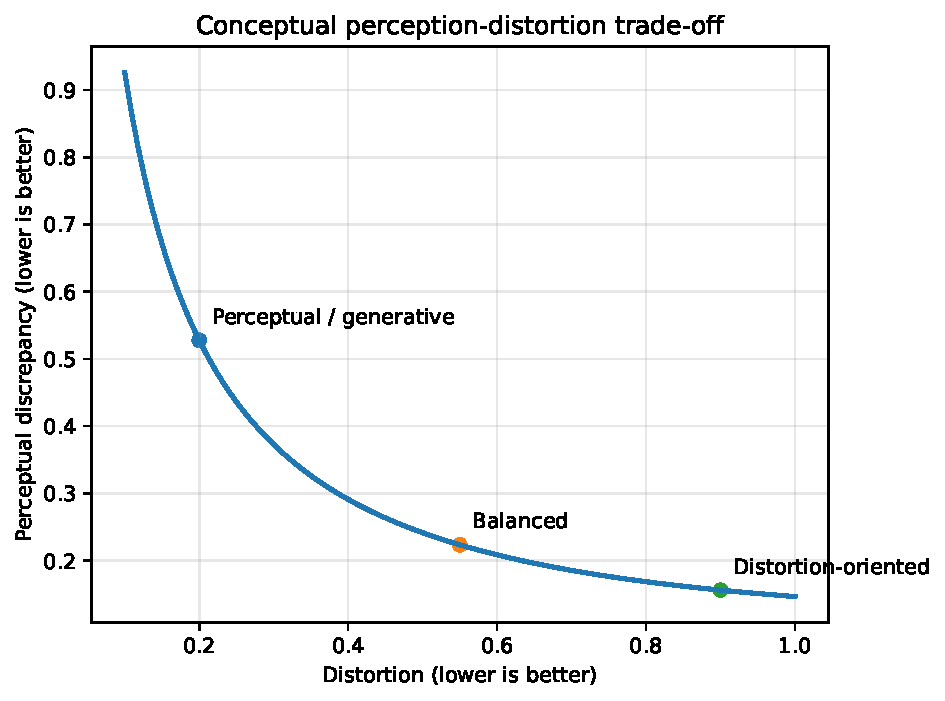
\includegraphics[width=.75\textwidth]{perception_distortion_tradeoff.pdf}
\caption{نمای مفهومی مبادله ادراک و اعوجاج. حرکت به سوی بافت طبیعی‌تر می‌تواند خطای نمونه‌به‌نمونه را افزایش دهد.}
\label{fig:perception-distortion}
\end{figure}

\begin{warningbox}
عبارت‌هایی مانند «جزئیات بازیابی شد» فقط زمانی مجازند که داده یا حقیقت مبنا از آن پشتیبانی کند. در غیر این صورت باید گفت
«جزئیات محتمل تولید شد» یا «کیفیت ادراکی افزایش یافت». این تفاوت در مقاله علمی حیاتی است.
\end{warningbox}

% =============================================================================
\section{ارزیابی: از \lr{PSNR} تا کار پایین‌دست و عدم‌قطعیت}
% =============================================================================

\subsection{معیارهای دارای مرجع}
برای دامنه شدت \([0,L]\):
\begin{align}
\MSE&=\frac1n\norm{\widehat x-x}^2,\\
\PSNR&=10\log_{10}\frac{L^2}{\MSE}.
\end{align}
\lr{SSIM} روشنایی، کنتراست و ساختار محلی را مقایسه می‌کند. معیارهای ویژگی‌محور مانند \lr{LPIPS} به شباهت ادراکی نزدیک‌ترند،
اما به شبکه ویژگی و داده آموزش آن وابسته‌اند.

\subsection{معیار سازگاری داده}
حتی با حقیقت مبنا باید
\begin{equation}
r=y-H\widehat x
\end{equation}
بررسی شود. برای مدل گاوسی سفید، باقیمانده باید تقریباً صفرمیانگین، با واریانس درست و بدون ساختار مکانی باشد.
وجود لبه در باقیمانده نشانه حذف جزئیات؛ وجود ساختار دوره‌ای نشانه مدل تاری یا مرز اشتباه است.

\subsection{کار پایین‌دست}
اگر خروجی برای قطعه‌بندی، تشخیص یا اندازه‌گیری استفاده می‌شود، عملکرد همان وظیفه باید گزارش شود.
ممکن است روش با \lr{PSNR} پایین‌تر، مرزهای تشخیصی را بهتر حفظ کند. در مقابل روش مولد ممکن است تصویر زیباتر ولی ویژگی کاذب بسازد.

\subsection{هزینه و پایداری}
گزارش کامل شامل زمان، حافظه، تعداد پارامتر، تعداد ارزیابی شبکه، انرژی تقریبی، حساسیت به اندازه تصویر و عملکرد روی دستگاه هدف است.
برای روش تکراری، تنها زمان یک تکرار کافی نیست؛ معیار توقف و تعداد واقعی تکرار باید ذکر شود.

\subsection{پروتکل داده واقعی}
\begin{enumerate}
\item داده خام و \lr{sRGB} را مخلوط نکنید؛
\item جداسازی آموزش/اعتبارسنجی/آزمون بر اساس صحنه و دستگاه انجام شود، نه وصله تصادفی از یک تصویر؛
\item تخریب مصنوعی باید زنجیره حسگر را تا حد ممکن بازنمایی کند؛
\item حداقل یک آزمون انتقال به سطح نویز، دوربین یا تخریب دیده‌نشده اجرا شود؛
\item تصاویر شکست و نه فقط بهترین نمونه‌ها منتشر شوند.
\end{enumerate}

\begin{figure}[H]
\centering
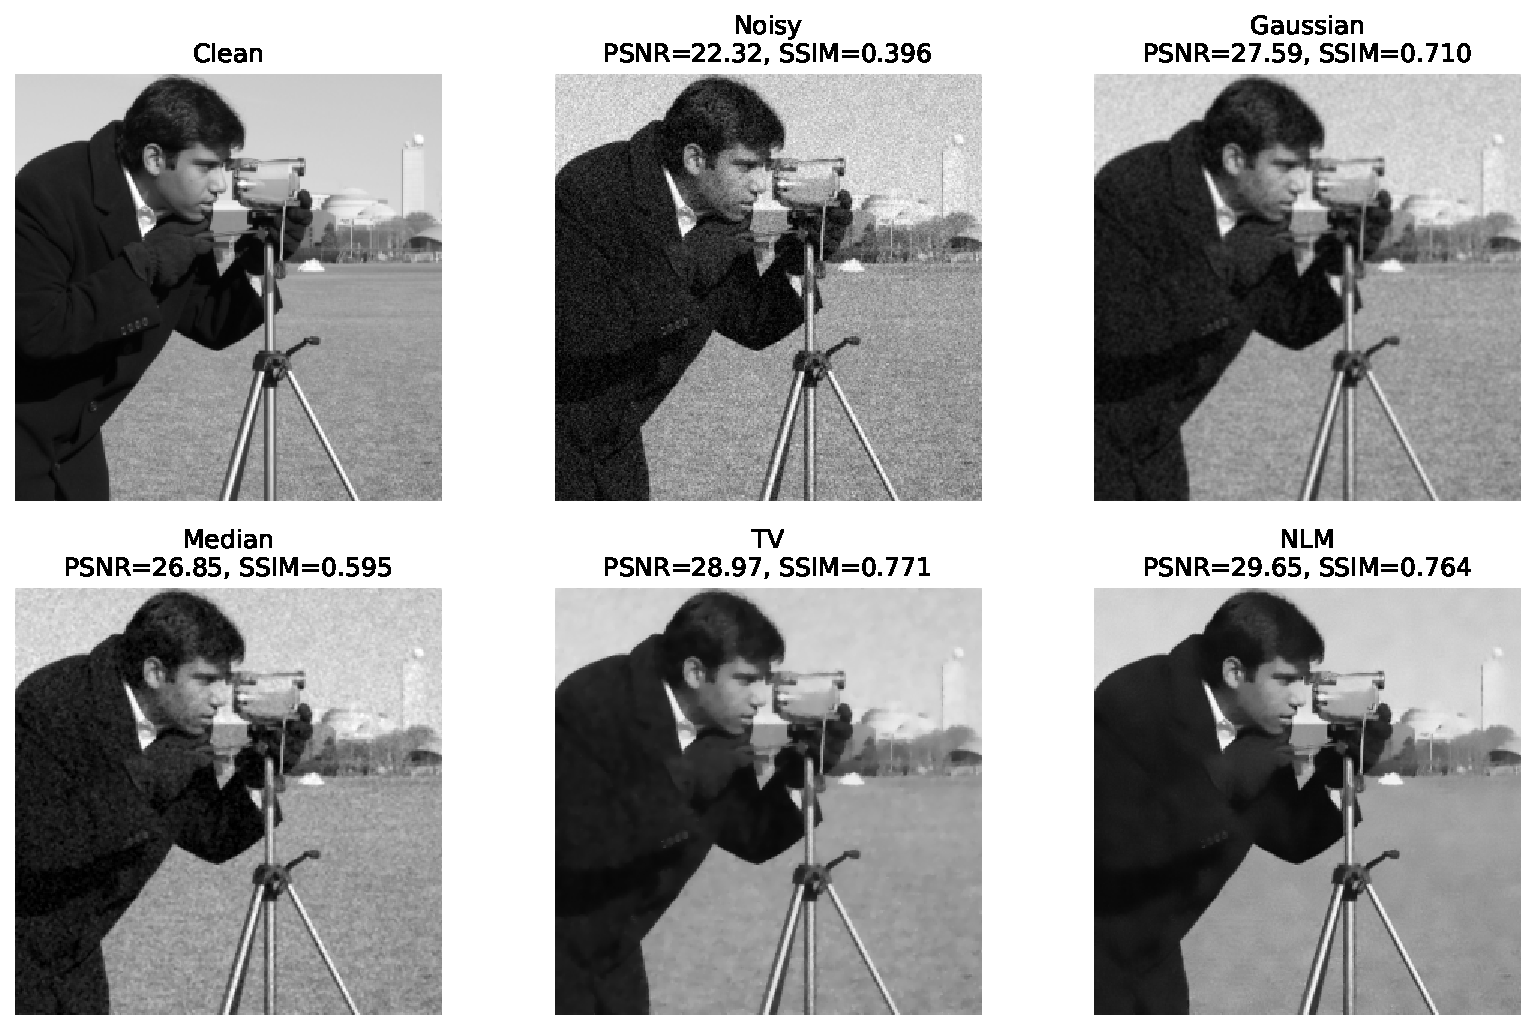
\includegraphics[width=.98\textwidth]{classical_denoising_comparison.pdf}
\caption{مقایسه بازتولیدپذیر چند خط مبنای کلاسیک روی نویز گاوسی مصنوعی. عدد بهتر همیشه به معنی بافت یا لبه بهتر در همه نواحی نیست.}
\label{fig:classical-comparison}
\end{figure}

% =============================================================================
\section{راهنمای انتخاب خانواده روش}
% =============================================================================

\begin{longtable}{>{\raggedleft\arraybackslash}p{3.1cm} >{\raggedleft\arraybackslash}p{3.5cm} >{\raggedleft\arraybackslash}p{3.5cm} >{\raggedleft\arraybackslash}p{3.7cm}}
\caption{راهنمای عملی انتخاب روش؛ این جدول جای آزمایش را نمی‌گیرد.}\\
\toprule
وضعیت & نقطه شروع مناسب & مزیت & هشدار \\
\midrule
\endfirsthead
\toprule
وضعیت & نقطه شروع مناسب & مزیت & هشدار \\
\midrule
\endhead
نویز گاوسی معلوم و نیاز به خط مبنا & وینر، موجک، \lr{BM3D}، \lr{TV} & قابل تفسیر و کم‌داده & مدل نویز واقعی ممکن است نقض شود \\
نویز ضربه‌ای & میانه، \(\ell_1\)، مدل متغیر پرت & مقاوم به پرت & بافت ریز ممکن است حذف شود \\
نویز وابسته به سیگنال & درست‌نمایی پواسون--گاوسی یا تثبیت واریانس & سازگار با حسگر & وارون‌سازی تبدیل و کالیبراسیون مهم است \\
رفع تاری با \lr{PSF} معلوم & وینر/تیکانوف، \lr{TV}، \lr{PnP} & قید داده صریح & مرز و خطای هسته \\
تخریب مجهول ولی داده زوجی زیاد & شبکه کور یا همه‌کاره & سرعت آزمون بالا & شکست خارج از توزیع \\
عملگر جدید و داده پاک کم & \lr{PnP}، شبکه بازشده، پیشین امتیاز & انتقال‌پذیری بیشتر & همگرایی و هزینه تکرار \\
مسئله چندجوابی & نمونه‌گیری پسین & نمایش عدم‌قطعیت & کالیبراسیون و توهم \\
کاربرد پزشکی/علمی & مدل فیزیکی + عدم‌قطعیت + آزمون باقیمانده & قابلیت ممیزی & تصویر زیبا معیار کافی نیست \\
سامانه لبه‌ای & مدل سبک، جدول جست‌وجو، فیلتر کلاسیک یا شبکه کوچک & تأخیر و انرژی کم & افت تعمیم و محدودیت دقت \\
\bottomrule
\end{longtable}

% =============================================================================
\section{کارگاه بازتولیدپذیر فصل}
% =============================================================================

\begin{workshopbox}[هدف]
یک آزمایش کامل باید نه فقط خروجی تصویری، بلکه مدل تخریب، سطح نویز، پارامتر انتخاب‌شده، معیارها، زمان، باقیمانده و نسخه نرم‌افزار را ثبت کند.
بسته این فصل اسکریپت تولید شکل‌ها و فایل‌های \lr{CSV} تحلیل حساسیت را شامل می‌شود.
\end{workshopbox}

\subsection{قرارداد داده و توابع پایه}
\begin{latin}
\begin{lstlisting}
from dataclasses import dataclass
import numpy as np
from skimage.metrics import peak_signal_noise_ratio, structural_similarity

@dataclass(frozen=True)
class GaussianNoise:
    sigma: float
    seed: int = 1405

    def apply(self, clean: np.ndarray) -> np.ndarray:
        if clean.dtype.kind != "f":
            raise TypeError("clean must be floating point in [0, 1]")
        rng = np.random.default_rng(self.seed)
        noisy = clean + rng.normal(0.0, self.sigma, clean.shape)
        return np.clip(noisy, 0.0, 1.0)

def metrics(clean: np.ndarray, estimate: np.ndarray) -> dict[str, float]:
    return {
        "psnr": float(peak_signal_noise_ratio(clean, estimate, data_range=1.0)),
        "ssim": float(structural_similarity(clean, estimate, data_range=1.0)),
        "mse": float(np.mean((clean - estimate) ** 2)),
    }
\end{lstlisting}
\end{latin}

\subsection{حل تیکانوف کانولوشنی در حوزه فوریه}
\begin{latin}
\begin{lstlisting}
import numpy as np
from scipy.fft import fft2, ifft2


def psf_to_otf(psf: np.ndarray, shape: tuple[int, int]) -> np.ndarray:
    """Embed and circularly shift a PSF to construct its OTF."""
    canvas = np.zeros(shape, dtype=float)
    h, w = psf.shape
    canvas[:h, :w] = psf
    canvas = np.roll(canvas, -(h // 2), axis=0)
    canvas = np.roll(canvas, -(w // 2), axis=1)
    return fft2(canvas)


def tikhonov_deblur(y: np.ndarray, psf: np.ndarray, lam: float) -> np.ndarray:
    if lam <= 0:
        raise ValueError("lam must be positive")
    H = psf_to_otf(psf / psf.sum(), y.shape)
    # First-order periodic finite differences
    dx = np.zeros(y.shape); dx[0, 0], dx[0, 1] = -1, 1
    dy = np.zeros(y.shape); dy[0, 0], dy[1, 0] = -1, 1
    Dx, Dy = fft2(dx), fft2(dy)
    denominator = np.abs(H) ** 2 + lam * (np.abs(Dx) ** 2 + np.abs(Dy) ** 2)
    X = np.conj(H) * fft2(y) / np.maximum(denominator, 1e-12)
    return np.real(ifft2(X))
\end{lstlisting}
\end{latin}

\subsection{گرادیان پروگزیمال و ثبت تاریخچه}
\begin{latin}
\begin{lstlisting}
from collections.abc import Callable
import numpy as np

Array = np.ndarray


def proximal_gradient(
    x0: Array,
    grad_f: Callable[[Array], Array],
    prox_g: Callable[[Array, float], Array],
    step: float,
    objective: Callable[[Array], float],
    max_iter: int = 300,
    tol: float = 1e-6,
) -> tuple[Array, list[float]]:
    if step <= 0:
        raise ValueError("step must be positive")
    x = x0.copy()
    history = [objective(x)]
    for _ in range(max_iter):
        x_next = prox_g(x - step * grad_f(x), step)
        history.append(objective(x_next))
        relative = np.linalg.norm(x_next - x) / max(np.linalg.norm(x), 1e-12)
        x = x_next
        if relative < tol:
            break
    return x, history
\end{lstlisting}
\end{latin}

\subsection{پروتکل مقایسه منصفانه}
\begin{enumerate}
\item سه سطح نویز و دست‌کم پنج تصویر با ساختار متفاوت؛
\item تنظیم پارامتر فقط روی اعتبارسنجی؛
\item اجرای چند بذر نویز و گزارش میانگین و انحراف معیار؛
\item ثبت \lr{PSNR}، \lr{SSIM}، زمان و معیار حفظ لبه؛
\item نمایش برش بزرگ‌نمایی‌شده و باقیمانده با مقیاس ثابت؛
\item آزمون حساسیت به خطای تخمین \(\sigma\)؛
\item یک آزمون داده واقعی یا تخریب خارج از مدل.
\end{enumerate}

\subsection{پرامپت دقیق برای Codex}
\begin{workshopbox}[پرامپت]
\begin{latin}
\small
Act as a research software engineer in inverse imaging. Build a fully reproducible Python
benchmark for Chapter 5. Use a clean package structure with typed functions, unit tests,
fixed random seeds, configuration files, CSV outputs, and publication-quality figures.
Implement: Gaussian/Poisson/impulse degradation; Gaussian and median filters; wavelet
soft thresholding; non-local means; TV denoising; Tikhonov deblurring; an ISTA/FISTA
solver; and one plug-and-play reconstruction using a clearly documented denoiser.
For every method, separate training/tuning/test information, record runtime and memory,
check data consistency, and report mean plus standard deviation over Monte Carlo trials.
Do not silently clip arrays or mix uint8 and floating-point intensity scales. Add tests for
adjoint consistency of $H$ and $H^T$, finite-difference gradient checks, reproducibility, and
boundary conditions. Produce a failure-case gallery and a Markdown report explaining
where each model assumption is violated. Do not fabricate results: execute every experiment.
\end{latin}
\end{workshopbox}

% =============================================================================
\section{تمرین‌های ریاضی، محاسباتی و پژوهشی}
% =============================================================================

\subsection*{تمرین‌های اثباتی}
\begin{enumerate}
\item رابطه وینر \eqref{eq:wiener} را با مشتق‌گیری مستقیم از \(\E|X-GY|^2\) استخراج کنید.
\item نشان دهید برای پیشین گاوسی و نویز گاوسی، \lr{MAP} و \lr{MMSE} یکسان‌اند.
\item پروگزیمال \(\lambda|x|\) را با بررسی سه حالت \(x>0\)، \(x<0\) و \(x=0\) به‌دست آورید.
\item دوگان تغییرات کلی همسانگرد را استخراج کنید و قید \(\norm{p_i}_2\le1\) را توضیح دهید.
\item ثابت کنید تیکانوف مرتبه صفر در پایه بردارهای منفرد ضریب فیلتری \(\sigma_i^2/(\sigma_i^2+\lambda)\) دارد.
\item برای مدل پواسون، گرادیان و هسین جمله داده \eqref{eq:poisson-data-term} را به‌دست آورید و محدب‌بودن را بررسی کنید.
\item شرطی ارائه کنید که یک نگاشت خطی \(D(x)=Wx\) پروگزیمال یک تابع محدب باشد.
\item هویت توییدی \eqref{eq:tweedie} را با مشتق‌گیری از کانولوشن چگالی با گاوسی اثبات کنید.
\end{enumerate}

\subsection*{تمرین‌های محاسباتی}
\begin{enumerate}
\item واریانس خروجی فیلترهای میانگین \(3\times3\)، \(5\times5\) و گاوسی را با رابطه \eqref{eq:filtered-noise-var} پیش‌بینی و تجربی تأیید کنید.
\item یک تصویر را با نویز نمک‌وفلفل و گاوسی تخریب کنید و میانگین و میانه را روی هر دو مقایسه کنید.
\item آستانه جهانی، \lr{SURE} و آستانه اعتبارسنجی را برای موجک مقایسه کنید.
\item پیاده‌سازی ساده \lr{NLM} بنویسید و اثر اندازه وصله، پنجره جست‌وجو و \(h\) را تحلیل کنید.
\item مدل \lr{ROF} را با روش اولیه--دوگان حل کنید و شکاف اولیه--دوگان را رسم کنید.
\item رفع تاری تیکانوف را با سه شرط مرزی پیاده‌سازی و مصنوعات مرزی را مقایسه کنید.
\item برای یک اپراتور \(H\) آزمون عددی الحاقی
\(\inner{Hx}{y}\approx\inner{x}{H^Ty}\) بنویسید.
\item در یک مسئله درون‌پرکردن، پنج نمونه مولد تولید کنید و واریانس نواحی مفقود و مشاهده‌شده را مقایسه کنید.
\end{enumerate}

\subsection*{تمرین‌های پژوهشی}
\begin{enumerate}
\item یک مقاله کلاسیک مانند \lr{BM3D} و یک مدل جدید مانند \lr{Restormer} را از نظر فرض، داده، هزینه، پیچیدگی و نوع شکست مقایسه کنید؛ نه فقط جدول \lr{PSNR}.
\item بررسی کنید آیا حذف‌کننده انتخابی شما تقریباً غیرانبساطی است. نسبت
\(\norm{D(x+\delta)-D(x)}/\norm{\delta}\) را برای اغتشاش‌های مختلف تخمین بزنید.
\item یک پروتکل برای تشخیص توهم در ابرتفکیک پزشکی یا ماهواره‌ای طراحی کنید.
\item یک روش همه‌کاره بازسازی را روی تخریب مرکب دیده‌نشده آزمایش کنید و بازنمایی تخریب را تحلیل نمایید.
\item یک روش نمونه‌گیری پسین را از نظر پوشش بازه، سازگاری داده و تنوع مؤثر ارزیابی کنید.
\item هزینه انرژی و تأخیر یک شبکه بزرگ را با \lr{BM3D}، \lr{TV} و یک شبکه سبک روی سخت‌افزار واقعی مقایسه کنید.
\end{enumerate}

% =============================================================================
\section{تقسیم پیشنهادی فصل به ویدئوهای ۱۵ دقیقه‌ای}
% =============================================================================

\begin{videobox}
\begin{enumerate}
\item \textbf{ویدئو ۱:} تفاوت بهبود، حذف نویز، بازسازی و وظیفه پایین‌دست.
\item \textbf{ویدئو ۲:} مدل پیشرو، درست‌نمایی و پیشین؛ استخراج انرژی \lr{MAP}.
\item \textbf{ویدئو ۳:} تابع خطر و اثبات برآوردگر میانگین شرطی.
\item \textbf{ویدئو ۴:} بدشرطی، \lr{SVD} و معنای منظم‌سازی طیفی.
\item \textbf{ویدئو ۵:} استخراج کامل فیلتر وینر و رابطه آن با تیکانوف.
\item \textbf{ویدئو ۶:} میانگین، میانه، دوطرفه و هدایت‌شده؛ حفظ لبه.
\item \textbf{ویدئو ۷:} موجک، تنکی، آستانه سخت و نرم و \lr{SURE}.
\item \textbf{ویدئو ۸:} خودشباهتی، \lr{NLM} و سوگیری فاصله وصله.
\item \textbf{ویدئو ۹:} گروه وصله، رتبه کم و معماری مفهومی \lr{BM3D}.
\item \textbf{ویدئو ۱۰:} مدل \lr{ROF}، معادله اویلر--لاگرانژ و پلکانی‌شدن.
\item \textbf{ویدئو ۱۱:} پروگزیمال و استخراج \lr{ISTA/FISTA}.
\item \textbf{ویدئو ۱۲:} \lr{ADMM}، باقیمانده‌ها و تنظیم پارامتر.
\item \textbf{ویدئو ۱۳:} رفع تاری، شرایط مرزی و رفع تاری کور.
\item \textbf{ویدئو ۱۴:} درون‌پرکردن و ابرتفکیک به‌عنوان مسائل چندجوابی.
\item \textbf{ویدئو ۱۵:} یادگیری باقیمانده، \lr{DnCNN} و اثر تابع هزینه.
\item \textbf{ویدئو ۱۶:} ترنسفورمرهای بازسازی و مدل‌های همه‌کاره.
\item \textbf{ویدئو ۱۷:} شبکه‌های بازشده و جداسازی سازگاری داده از پیشین.
\item \textbf{ویدئو ۱۸:} \lr{Plug-and-Play}، \lr{RED} و مسئله همگرایی.
\item \textbf{ویدئو ۱۹:} هویت توییدی، تابع امتیاز و بازسازی با انتشار.
\item \textbf{ویدئو ۲۰:} نمونه‌گیری پسین، عدم‌قطعیت و خطر توهم.
\item \textbf{ویدئو ۲۱:} ادراک--اعوجاج، \lr{PSNR/SSIM/LPIPS} و معیار پایین‌دست.
\item \textbf{ویدئو ۲۲:} کارگاه مقایسه کلاسیک و تحلیل حساسیت پارامتر.
\item \textbf{ویدئو ۲۳:} طراحی آزمایش داده واقعی و آزمون خارج از توزیع.
\item \textbf{ویدئو ۲۴:} جمع‌بندی، نقد مقاله و تعریف پروژه پایان فصل.
\end{enumerate}
\end{videobox}

% =============================================================================
\section{پروژه پایان فصل: از مدل تا گزارش قابل داوری}
% =============================================================================

دانشجو یکی از سه مسیر را انتخاب می‌کند:
\begin{enumerate}
\item \textbf{مسیر کلاسیک عمیق:} مقایسه وینر، موجک، \lr{NLM}، \lr{BM3D} و \lr{TV} با تحلیل فرض و پیچیدگی؛
\item \textbf{مسیر ترکیبی:} بازسازی یک عملگر جدید با \lr{PnP} یا شبکه بازشده؛
\item \textbf{مسیر مولد:} نمونه‌گیری پسین برای درون‌پرکردن یا ابرتفکیک همراه با سنجش عدم‌قطعیت.
\end{enumerate}
گزارش باید شامل مدل پیشرو، مدل نویز، داده، معیار، خط مبنا، تنظیم پارامتر، تحلیل شکست، هزینه محاسباتی، کد و بذر تصادفی باشد.
حداقل یک ادعای کیفی باید با آزمون کمی یا تحلیل باقیمانده پشتیبانی شود.

% =============================================================================
\section{جمع‌بندی و پل به فصل ششم}
% =============================================================================

\begin{summarybox}
\begin{enumerate}
\item حذف نویز حالت ویژه‌ای از مسئله معکوس است؛ عملگر \(H\)، درست‌نمایی و پیشین باید از ابتدا روشن باشند.
\item برآوردگر بهینه به تابع خطر وابسته است: هزینه مربعی میانگین شرطی و هزینه قدرمطلق میانه شرطی را می‌دهد.
\item وینر راه‌حل خطی \lr{MMSE} است و تیکانوف همان منطق پایداری را از دیدگاه تغییراتی و بیزی بیان می‌کند.
\item روش‌های موجک، فرهنگ لغت، غیرمحلی و رتبه کم همگی درجه آزادی مؤثر تصویر را کاهش می‌دهند، اما با ساختارهای متفاوت.
\item \lr{TV} لبه را بهتر از همواری درجه دوم حفظ می‌کند، ولی فرض قطعه‌ای ثابت و پدیده پلکانی دارد.
\item روش‌های پروگزیمال زبان محاسباتی منظم‌سازهای ناهموارند و باید با شرط گام، باقیمانده و معیار توقف تدریس شوند.
\item شبکه‌های عمیق تابع شرطی را از داده می‌آموزند؛ نوع هزینه، داده آموزشی و تخریب شبیه‌سازی‌شده ماهیت برآوردگر را تعیین می‌کند.
\item شبکه بازشده و \lr{PnP} سازگاری فیزیکی را با پیشین آموخته‌شده ترکیب می‌کنند، اما تفسیر انرژی و همگرایی نیازمند شرط است.
\item مدل انتشار امکان نمونه‌گیری از پاسخ‌های متعدد را فراهم می‌کند، ولی بدون قید داده و کالیبراسیون ممکن است جزئیات کاذب بسازد.
\item ارزیابی معتبر باید هم‌زمان اعوجاج، ادراک، سازگاری داده، عدم‌قطعیت، هزینه و عملکرد پایین‌دست را بسنجد.
\item فصل ششم می‌تواند بر استخراج ویژگی، لبه، ساختار چندمقیاسی و نمایش‌های هندسی بنا شود؛ زیرا اکنون می‌دانیم پیش‌پردازش چگونه اطلاعات را حفظ یا نابود می‌کند.
\end{enumerate}
\end{summarybox}

\backmatter
\chapter*{منابع منتخب فصل}
\addcontentsline{toc}{chapter}{منابع منتخب فصل}

\begin{latin}
\begin{thebibliography}{99}

\bibitem{gonzalez}
R. C. Gonzalez and R. E. Woods,
\textit{Digital Image Processing}, 4th ed., Pearson, 2018.

\bibitem{bertero}
M. Bertero and P. Boccacci,
\textit{Introduction to Inverse Problems in Imaging}, CRC Press, 1998.

\bibitem{engl}
H. W. Engl, M. Hanke, and A. Neubauer,
\textit{Regularization of Inverse Problems}, Springer, 1996.

\bibitem{kay}
S. M. Kay,
\textit{Fundamentals of Statistical Signal Processing: Estimation Theory}, Prentice Hall, 1993.

\bibitem{wiener}
N. Wiener,
\textit{Extrapolation, Interpolation, and Smoothing of Stationary Time Series}, MIT Press, 1949.

\bibitem{tikhonov}
A. N. Tikhonov and V. Y. Arsenin,
\textit{Solutions of Ill-Posed Problems}, Winston, 1977.

\bibitem{rudin1992tv}
L. I. Rudin, S. Osher, and E. Fatemi,
``Nonlinear total variation based noise removal algorithms,''
\textit{Physica D}, vol. 60, pp. 259--268, 1992.

\bibitem{chambolle2004}
A. Chambolle,
``An algorithm for total variation minimization and applications,''
\textit{Journal of Mathematical Imaging and Vision}, vol. 20, pp. 89--97, 2004.

\bibitem{chambolle2011pd}
A. Chambolle and T. Pock,
``A first-order primal-dual algorithm for convex problems with applications to imaging,''
\textit{Journal of Mathematical Imaging and Vision}, vol. 40, pp. 120--145, 2011.

\bibitem{beck2009fista}
A. Beck and M. Teboulle,
``A fast iterative shrinkage-thresholding algorithm for linear inverse problems,''
\textit{SIAM Journal on Imaging Sciences}, vol. 2, no. 1, pp. 183--202, 2009.

\bibitem{boyd2011admm}
S. Boyd, N. Parikh, E. Chu, B. Peleato, and J. Eckstein,
``Distributed optimization and statistical learning via the alternating direction method of multipliers,''
\textit{Foundations and Trends in Machine Learning}, vol. 3, no. 1, pp. 1--122, 2011.

\bibitem{donoho1995wavelet}
D. L. Donoho,
``De-noising by soft-thresholding,''
\textit{IEEE Transactions on Information Theory}, vol. 41, no. 3, pp. 613--627, 1995.

\bibitem{stein1981sure}
C. M. Stein,
``Estimation of the mean of a multivariate normal distribution,''
\textit{The Annals of Statistics}, vol. 9, no. 6, pp. 1135--1151, 1981.

\bibitem{buades2005nlm}
A. Buades, B. Coll, and J.-M. Morel,
``A non-local algorithm for image denoising,''
in \textit{Proceedings of CVPR}, pp. 60--65, 2005.

\bibitem{dabov2007bm3d}
K. Dabov, A. Foi, V. Katkovnik, and K. Egiazarian,
``Image denoising by sparse 3-D transform-domain collaborative filtering,''
\textit{IEEE Transactions on Image Processing}, vol. 16, no. 8, pp. 2080--2095, 2007.

\bibitem{elad2006ksvd}
M. Aharon, M. Elad, and A. Bruckstein,
``K-SVD: An algorithm for designing overcomplete dictionaries for sparse representation,''
\textit{IEEE Transactions on Signal Processing}, vol. 54, no. 11, pp. 4311--4322, 2006.

\bibitem{candes2011rpca}
E. J. Candès, X. Li, Y. Ma, and J. Wright,
``Robust principal component analysis?,''
\textit{Journal of the ACM}, vol. 58, no. 3, 2011.

\bibitem{zhang2017dncnn}
K. Zhang, W. Zuo, Y. Chen, D. Meng, and L. Zhang,
``Beyond a Gaussian denoiser: Residual learning of deep CNN for image denoising,''
\textit{IEEE Transactions on Image Processing}, vol. 26, no. 7, pp. 3142--3155, 2017.

\bibitem{ulyanov2018dip}
D. Ulyanov, A. Vedaldi, and V. Lempitsky,
``Deep image prior,''
in \textit{Proceedings of CVPR}, pp. 9446--9454, 2018.

\bibitem{lehtinen2018n2n}
J. Lehtinen et al.,
``Noise2Noise: Learning image restoration without clean data,''
in \textit{Proceedings of ICML}, pp. 2965--2974, 2018.

\bibitem{batson2019n2s}
J. Batson and L. Royer,
``Noise2Self: Blind denoising by self-supervision,''
in \textit{Proceedings of ICML}, pp. 524--533, 2019.

\bibitem{venkatakrishnan2013pnp}
S. V. Venkatakrishnan, C. A. Bouman, and B. Wohlberg,
``Plug-and-play priors for model based reconstruction,''
in \textit{IEEE GlobalSIP}, pp. 945--948, 2013.

\bibitem{romano2017red}
Y. Romano, M. Elad, and P. Milanfar,
``The little engine that could: Regularization by denoising (RED),''
\textit{SIAM Journal on Imaging Sciences}, vol. 10, no. 4, pp. 1804--1844, 2017.

\bibitem{liu2021recovery}
J. Liu, Y. Sun, X. Xu, and U. S. Kamilov,
``Recovery analysis for plug-and-play priors using the restricted eigenvalue condition,''
in \textit{Advances in Neural Information Processing Systems}, 2021.

\bibitem{liang2021swinir}
J. Liang et al.,
``SwinIR: Image restoration using Swin Transformer,''
in \textit{Proceedings of ICCV Workshops}, pp. 1833--1844, 2021.

\bibitem{zamir2022restormer}
S. W. Zamir et al.,
``Restormer: Efficient Transformer for high-resolution image restoration,''
in \textit{Proceedings of CVPR}, pp. 5728--5739, 2022.

\bibitem{chen2022nafnet}
L. Chen, X. Chu, X. Zhang, and J. Sun,
``Simple baselines for image restoration,''
in \textit{Proceedings of ECCV}, pp. 17--33, 2022.

\bibitem{potlapalli2023promptir}
V. Potlapalli, S. W. Zamir, S. Khan, and F. S. Khan,
``PromptIR: Prompting for all-in-one blind image restoration,''
in \textit{Advances in Neural Information Processing Systems}, 2023.

\bibitem{li2025foundir}
H. Li, X. Chen, J. Dong, J. Tang, and J. Pan,
``FoundIR: Unleashing million-scale training data to advance foundation models for image restoration,''
in \textit{Proceedings of ICCV}, pp. 12626--12636, 2025.

\bibitem{song2021score}
Y. Song et al.,
``Score-based generative modeling through stochastic differential equations,''
in \textit{Proceedings of ICLR}, 2021.

\bibitem{chung2023dps}
H. Chung, J. Kim, M. T. Mccann, M. L. Klasky, and J. C. Ye,
``Diffusion posterior sampling for general noisy inverse problems,''
in \textit{Proceedings of ICLR}, 2023.

\bibitem{blau2018perception}
Y. Blau and T. Michaeli,
``The perception-distortion tradeoff,''
in \textit{Proceedings of CVPR}, pp. 6228--6237, 2018.

\bibitem{abdelhamed2018sidd}
A. Abdelhamed, S. Lin, and M. S. Brown,
``A high-quality denoising dataset for smartphone cameras,''
in \textit{Proceedings of CVPR}, pp. 1692--1700, 2018.

\bibitem{plotz2017dnd}
T. Plötz and S. Roth,
``Benchmarking denoising algorithms with real photographs,''
in \textit{Proceedings of CVPR}, pp. 1586--1595, 2017.

\bibitem{brooks2019unprocessing}
T. Brooks, B. Mildenhall, T. Xue, J. Chen, D. Sharlet, and J. T. Barron,
``Unprocessing images for learned raw denoising,''
in \textit{Proceedings of CVPR}, pp. 11036--11045, 2019.

\end{thebibliography}
\end{latin}

\chapter*{راهنمای کامپایل، فونت و اجرای آزمایش‌ها}
\addcontentsline{toc}{chapter}{راهنمای کامپایل، فونت و اجرای آزمایش‌ها}

فایل با \lr{XeLaTeX} کامپایل می‌شود. در \lr{TeXstudio}، کامپایلر پیش‌فرض را روی \lr{XeLaTeX} قرار دهید و برای تکمیل فهرست مطالب دو بار اجرا کنید.
فونت اصلی \lr{Amiri}، فونت لاتین \lr{DejaVu Serif} و فونت کد \lr{DejaVu Sans Mono} است؛ برای هر سه جایگزین خودکار تعریف شده است.
هیچ فایل فونتی در بسته قرار نگرفته است.

برای تولید شکل‌ها:
\begin{latin}
\begin{lstlisting}[language=bash]
python -m venv .venv
# Windows: .venv\Scripts\activate
# Linux/macOS: source .venv/bin/activate
pip install -r requirements.txt
python scripts/generate_figures.py
xelatex image_processing_next_decade_ch05_fa.tex
xelatex image_processing_next_decade_ch05_fa.tex
\end{lstlisting}
\end{latin}

\end{document}
